\documentclass{scrartcl}
\usepackage{graphicx}
\usepackage{array}
\usepackage[
    backend=biber,
    style=alphabetic,
    sorting=ynt
]{biblatex}
\usepackage{hyperref}
\usepackage{wrapfig}

\addbibresource{references.bib}

\title{Signal processing and Analysis of human brain potentials (EEG)}
\subtitle{Report}
\author{Felix Grüb, 3530441\\Simon Schindler, 3538650}
\date{\today}

\begin{document}

\maketitle

\vfill
Source files: \href{https://github.com/Feleuxens/Signal-Evaluation-and-EEG-Analysis-Grueb-Schindler}{github.com/Feleuxens/Signal-Evaluation-and-EEG-Analysis-Grueb-Schindler}

\newpage
\section*{Abstract}
This report presents a replication of the EEG/ERP analysis from Makin et al. (2012) \cite{paper}, who investigated symmetry perception using combined EEG and EMG. We developed a fully automated preprocessing pipeline, replacing the authors' manual inspection steps by using variance-based bad channel detection, bandpass and notch filtering, average rereferencing, Artifact Subspace Reconstruction (ASR), ICA-based artifact removal, interpolation, epoching, and amplitude-based trial rejection. We analyzed 24 subjects using 64-channel EEG data with reflectional symmetry and random pattern stimuli. Our pipeline successfully reproduced the general ERP morphology at PO7/PO8, including the P1, N1, and sustained posterior negativity (SPN) components. However, we found that ASR substantially attenuated the SPN difference between conditions. A follow-up analysis using automatic blink detection revealed that blink-contaminated epochs contribute to, but do not fully explain, this attenuation. We discuss the impact of each preprocessing step and the implications of ASR for ERP research on visual symmetry.

\newpage
\tableofcontents
\newpage

\section{Original Paper}
We chose the paper on symmetry perception since we had decided pretty early that we wanted to do something with the visual system.
We chose this paper over the others because it had quite a lot of data for us to work on and provided decent information on what they did and what they were looking for.
This was pretty important to us since we have never before worked with anything related to EEG-Data.

\subsection{Research question}
The paper from Makin. et al. \cite{paper} tried to do further experiments in the realm of symmetry perception.
Prior EEG studies reported symmetry-related ERPs (e.g., a sustained posterior negativity for symmetrical vs. random patterns) but concluded aesthetic evaluation requires explicit intent. 
This paper now combines ERP analysis with facial EMG and directly compares reflectional and rotational symmetry using specific patterns designed for this experiment.
Their main focus was on the question of whether these symmetry perception tasks are deliberate or automatic pre-attentive tasks.
To test their hypothesis, they used their patterns as stimuli and looked for the ERP responses.

The main research questions relevant to our further work here were:
\begin{itemize}
    \item Can the ERP effects reported by Makin et al. \cite{paper}, notably N1 sensitivity to regularity and P1 sensitivity to rotational symmetry, be reproduced when closely matching their stimuli, task, and preprocessing/analysis pipeline?
    \item Focused ERP aims: replicate and quantify effect sizes and scalp topographies for P1, N1, and the sustained posterior negativity (SPN); assess timing differences between reflectional and rotational symmetry; and determine whether task-driven attentional biases could explain early ERP differences.
\end{itemize}

Overview of replicated EEG/ERP approach
\begin{itemize}
    \item Stimuli: trial-unique quadrant-based black-and-white patterns (reflectional, rotational, random) matched for density, numerosity, contrast, and luminance so that global inter-quadrant relations determine regularity.
    \item Task: speeded classification to ensure attention to global regularity.
    \item Recording: continuous EEG (64-channel, 10–20 montage) with posterior electrode focus.
    \item Preprocessing: bandpass filtering, ICA for ocular/muscle artifacts, epoching, baseline correction.
    \item ERP windows: P1 (100–130 ms), N1 (170–200 ms), and sustained posterior negativity (300–1000 ms).
    \item Statistics: within-subject comparisons, repeated-measures ANOVAs, cluster/FDR correction, effect sizes, and scalp topographies.
\end{itemize}

Our main focus for our replication lies in their Experiment 1.
In this experiment, they analyzed the difference between two stimulus types: two-fold reflectional symmetry and equivalent random patterns.
For each stimulus, its crafted patterns with specific backgrounds, etc., were presented to the subject for 3s each.
While the subject had to analyze the pattern and decide whether it was symetric or random, they recorded EEG and facial EMG of: left Zygomaticus Major (ZM) and left Corrugator Supercilii (CS) recorded with standard bipolar electrode placements. VEOG and HEOG recorded for blink/eye-movement detection.

For the experiment itself, each subject was shown shapes (reflection, random), 80 trials per condition, with a randomized trial order.
Each trial had a timing:
\begin{enumerate}
    \item 1.5 s fixation baseline
    \item 3 s pattern presentation
    \item response screen (up to 3 s to respond)
\end{enumerate}
They also included practice blocks of 16 trials with given feedback to eliminate further unwanted side effects.



\subsection{Authors Pipeline}
The analysis of the EEG data is described by the authors in their paper~\cite{paper}.
The relevant parts for our further work are the following:
\begin{table}[h]
    \centering
    \begin{tabular}{|l|l|}
    \hline
        Bad Channel detection & manual inspection by the authors \\
        Lowpass filter & $25$ Hz \\
        Highpass filter & None specified in the paper \\
        50Hz filter & Nothing specified. We suspect none \\
        Downsampling & $512$ to $128$ Hz \\
        Artefact removal & ICA implementation without further details \\
        Interpolation & Nothing specified \\
        Epochs & $-1$ to $1$ sec \\
        Averaging & Not directly specified but suspected mean \\
        Baseline correction & $-200$ to $+50$ ms Mean baseline subtraction \\
        Trial rejection & $\pm 100$mV before ICA, $\pm75$mV after ICA \\
        \hline
    \end{tabular}
    \caption{Author's pipeline}
\end{table}


\section{Our Pipeline Overview}\label{pipeline}
In contrast to the author's pipeline, we wanted to achieve similar results but with differing pipelines.
The greatest difference is our choice to include ASR in our Pipeline which the authors did not use.
From our first understanding, this should only be better since we clean our data even more.
We also put our focus on an automatic pipeline instead of doing manual steps.

\begin{table}[h]
    \hspace*{-1.8cm}\begin{tabular}{|l|l|l|}
        \hline
         & authors pipeline & our pipeline \\
        \hline
        Bad Channel detection & manual inspection by the authors & Variance z-score, Low-correlation \\
        Lowpass filter & $25$ Hz & $40$ Hz \\
        Highpass filter & None specified in the paper & $0.1$ Hz \\
        50Hz filter & Nothing specified. We suspect none & Notch \\
        Downsampling & $512$ to $128$ Hz & $512$ to $128$ Hz \\
        Artefact removal & ICA implementation without further details & ASR + ICA \\
        Interpolation & Nothing specified & mne-accurate for all bads \\
        Epochs & $-1$ to $1$ sec & $-0.5$ to $1$ sec \\
        Averaging & Not directly specified but suspected mean & grand average \\
        Baseline correction & $-200$ to $+50$ ms mean baseline subtraction & $-250$ to $0$ ms mean baseline subtraction \\
        Trial rejection & $\pm 100$mV before ICA, $\pm 75$mV after ICA & $\pm 100$mv at the end \\
        \hline
    \end{tabular}
    \caption{The author's pipeline compared to our pipeline}
    \label{tab:pipeline}
\end{table}

In the following, we are going into each of the subsequent steps and talking about our decision-making and why we chose what we used.

\subsection{Step01 Loading}
For loading all the data, we just had to use the \texttt{mne}-package and load the already correctly organized data in BIDS format.
There is nothing really special in this step.

\subsection{Step02 Bad Channels}
The authors did a manual inspection of their collected data.
We wanted to go a different route here for multiple reasons.
Although we have seen some examples and a high-level explanation of what artefacts are and look like, we are in no way practiced or experienced in detecting all kinds of artefacts or problems in the EEG-data.
Secondly, we are studying computer science and therefore clearly favor automatic solutions, where the computer does the necessary computations.

From these two aspects, it was clear to us that we wanted to use some kind of automatic bad-channel detection.
Through the lecture and online resources, we stumbled upon a pretty easy solution to just calculate variances and correlations of channels. With that, we can detect channels with high variance and low correlation and mark them as \texttt{bad} in the EEG data.

We set the z-score threshold to 3.0 for both detection methods. A z-score of 3 corresponds roughly to the 99.7th percentile under a normal distribution, meaning only channels whose variance or correlation deviates by more than three standard deviations from the mean are flagged. This is a conservative choice that avoids marking borderline channels as bad while still catching clearly problematic ones. More aggressive thresholds (e.g., 2.0) risk excluding channels that are merely noisy but still carry usable signal, which would reduce spatial coverage and degrade interpolation quality later.

\subsection{Step03 Filtering}
In their paper, the authors used only a 25Hz low-pass filter as far as we could tell. Also, nothing was mentioned about a 50Hz filter in any way.

We wanted to go a different route and definitely wanted to filter a bit more. Partially because we expected our automatic filtering to maybe be a bit worse than their manual inspections. For the bandpass filter, we chose a high-pass cutoff of 0.1 Hz and a low-pass cutoff of 40 Hz. The 0.1 Hz high-pass removes slow drifts and DC offsets while preserving the slow components relevant to our ERP analysis, particularly the sustained posterior negativity which extends over several hundred milliseconds. A more aggressive high-pass (e.g., 1 Hz) would improve ICA decomposition quality but risks attenuating slow ERP components. The 40 Hz low-pass is more permissive than the authors' 25 Hz but still removes high-frequency muscle artifacts and line noise harmonics above the first. We chose 40 Hz to retain more of the original signal, relying on the notch filter to handle 50 Hz line noise specifically.

For the notch filter, we targeted 50 Hz and its harmonics at 100, 150, and 200 Hz, as these are the expected power line interference frequencies in Europe. As discussed in the lecture, using a Notch filter for filtering possible 50Hz noise is reasonable since it doesn't hurt really, even tho we could mostly not identify 50Hz noise in the recorded data. We used the spectrum\_fit method, which estimates and subtracts the line noise component without the spectral distortion that a simple notch filter can introduce at neighboring frequencies. We applied both filters only to EEG channels, leaving EOG and misc channels unfiltered to preserve their full signal for later artifact detection in the ICA step.

\subsection{Step04 Downsampling}
In the beginning, other than the authors, we did not plan to downsample the recorded data at 512 Hz.
We didn't really have a need and just expected the pipeline to run a bit longer since there are more datapoints.

But quickly we ran into problems when implementing the following ASR step.
When using ASR, even on our Machines with 32GB of RAM, we crashed with in Seconds of ASR running, because of excessive Memory usage.
That's why we then also went the route of downsampling to 128 Hz which seems to be a reasonable sampling rate from what we have seen.

\subsection{Step05 Rereferencing}
After filtering and downsampling, we re-referenced the EEG data to the average of all EEG channels. Average referencing is a standard choice in ERP research as it reduces the influence of any single reference electrode and provides a reference-free representation of the scalp potential distribution. We chose average referencing over other common options (e.g., linked mastoids or Cz) because it does not privilege any single electrode and provides a reference-free approximation of the scalp potential. This is particularly important for our analysis at PO7/PO8, as an asymmetric reference could introduce bias between hemispheres. We set projection to False, meaning the re-referencing is applied directly to the data rather than stored as a projector, ensuring all subsequent steps operate on the actual re-referenced values.

 This step had one of the largest impacts on our results (see Section \ref{impact-steps}), as it removes shared noise across all channels, substantially cleaning the grand average ERP waveforms. We used mne's built-in \texttt{set\_eeg\_reference} with the average setting. Importantly, average rereferencing reduces the rank of the data by one, which we accounted for in the subsequent ICA step by computing the data rank and setting the number of ICA components accordingly. 

\subsection{Step06 ASR}
Other than the Authors, we wanted to look into ASR since it was introduced in the lecture and seemed not to be as popular anymore/at all. We used the asrpy package, a Python implementation of Artifact Subspace Reconstruction as the \texttt{mne}-package doesn't implement ASR. ASR works by first identifying clean calibration segments in the continuous data, computing a covariance matrix from these segments, and then reconstructing time windows whose signal subspace deviates too far from this clean reference. The key parameter is the cutoff threshold, which we set to 10 (the default in most implementations) \cite{asr-parameters}. Lower values (e.g., 5) result in more aggressive artifact removal, while higher values (e.g., 20) are more permissive. We tested cutoff values of 5, 10, and 20 and found the impact of this parameter to be relatively minor compared to the binary choice of enabling or disabling ASR entirely (see Section \ref{asr-parameters}). One practical challenge we encountered was memory consumption: at the original 512 Hz sampling rate, ASR exceeded 32 GB of RAM, which motivated our decision to downsample to 128 Hz before this step. Additionally, ASR failed on some subjects due to insufficient clean calibration data, in which case the pipeline continued without ASR for those subjects.

\subsection{Step07 ICA}
For artifact removal beyond ASR, we applied Independent Component Analysis (ICA) using the Infomax algorithm. ICA decomposes the multichannel EEG signal into statistically independent components, allowing identification and removal of components corresponding to ocular and cardiac artifacts. We chose the Infomax algorithm because it is the most widely used ICA method in EEG research and the default in both EEGLAB and MNE. Infomax assumes super-Gaussian source distributions, which is a reasonable assumption for the types of artifacts we aimed to remove (eye blinks, eye movements, and cardiac activity). We initially set n\_components to 0.99, meaning PCA would retain components explaining 99 \% of the variance before ICA decomposition. However, we encountered numerical issues on several subjects where average re-referencing and bad channel exclusion had reduced the effective data rank, causing a single PCA component to capture nearly all variance. To resolve this, we computed the actual matrix rank of the data and set n\_components to rank minus one. This approach is recommended by MNE's documentation for rank-deficient data and ensures stable ICA decomposition regardless of the number of excluded channels or the reference scheme used. For automatic component identification, we relied on MNE's correlation-based methods (find\_bads\_eog and find\_bads\_ecg), which correlate each component's time course with the EOG and ECG channels respectively and flag components exceeding a correlation threshold.

\subsection{Step08 Interpolation}
Since we did detect bad-channels at the beginning of the pipeline, we now want to reconstruct them using interpolation. We excluded bad-channels from the steps above, since they would cause possible problems, especially in running ICA and detecting independent components. Also we want to interpolate from the cleanest data we have and therefore do this step as late in the pipeline as possible.

We used MNE's "accurate" interpolation mode, which implements spherical spline interpolation as described by Perrin et al. \cite{interpolation}. This method models the scalp as a sphere and fits a smooth spline surface through the remaining good channels to estimate the missing channel's signal. Compared to the "fast" mode, which uses a simpler nearest-neighbor approach, spherical splines produce more physically plausible reconstructions but are computationally more expensive. Given our relatively small number of bad channels (typically one to three per subject), the additional computation was negligible. 

\subsection{Step09 Epoching}
For epoching the processed channels, we also use the built in functionallity. We went for a bit shorter epochs than the authors in their paper. We chose a baseline window of -250 to 0 ms rather than the authors' -200 to +50 ms. Our window is entirely pre-stimulus, which avoids any contamination of the baseline by early visual processing (the P1 begins around 80-100 ms). Our 250 ms window is long enough to provide a stable estimate of the pre-stimulus mean while staying within our epoch boundary of -500 ms.
One second seemed to be reasonable to as, as the authors used the same, and we have seen visual stimuli in the lecture and from what we have learned, all the characteristics of visual stimuli are present way earlier than one second after the event.

\subsection{Step10 Trialrejection}
Our EEG threshold of $150 \mu V$ is a compromise between the authors' two-pass approach ($100 \mu V$ before ICA, $75 \mu V$ after). Since we apply rejection only once at the end of the pipeline, after both ASR and ICA have already cleaned the data, a single moderate threshold captures remaining artifacts without being overly aggressive. The $250 \mu V$ EOG threshold is more permissive than the EEG threshold because EOG channels naturally have higher amplitudes due to their proximity to the eyes; rejecting at the same threshold as EEG would discard too many usable epochs. The flat threshold of $1 \mu V$ catches epochs where a channel was effectively disconnected or produced constant output, which would otherwise distort the average. These values are consistent with commonly used thresholds in the MNE documentation and other published ERP pipelines.


\subsection{Plotting}
Finally, we accumulated all the epochs we got from our pipelines and used a Grand Average across PO7 and PO8, just like the authors, and plotted our results the same way as theirs to make it easy to compare results.

\subsection{Implementation Details}
To easily run different variations of the pipeline, we introduced configurations files with which parameters for each step can be set as well as enabling or skipping entire steps. Using the toml layout, each step has its own section in the config file enabling easy, type-safe loading of the parameters.

Additionally, we introduced parallelization using the multiprocessing package to speed up the data processing by executing the pipeline on multiple subjects concurrently.


\section{Results}
In this section, we compare the authors' reported ERP results with our own. Both analyses focus on the grand average ERP at electrodes PO7 and PO8, examining the P1 (100-130 ms), N1 (170-200 ms), and sustained posterior negativity (SPN, 300-1000 ms) for reflectional symmetry versus random patterns across all 24 subjects. Note that our baseline correction window (-250 to 0 ms) differs from the authors' (-200 to +50 ms), which may affect absolute amplitude comparisons.

\subsection{Authors results}
As stated by the authors, their ERP data revealed several instructive similarities and differences from previous work. 
They found the N1 amplitude to be greater for reflection patterns.
According to them, this suggests visual symmetry detection begins at an earlier stage in visual processing than previously thought~\cite{humansymetry}.
This could be because the background did not appear at the same time as the pattern elements in our Experiment 1, while this could
have masked N1 modulations in previous studies. 

Additionally, the authors noted that they did replicate the sustained posterior negativity reported by other authors.
They further analyzed these patterns and used source localization using LORETA and identified generators in the extrastriate visual cortex, consistent with previous neuroimaging work.

Relevant to our further work is mostly how the combined average of PO7 and PO8 behaved.

\begin{center}
    \begin{figure}[h]
        \centering
        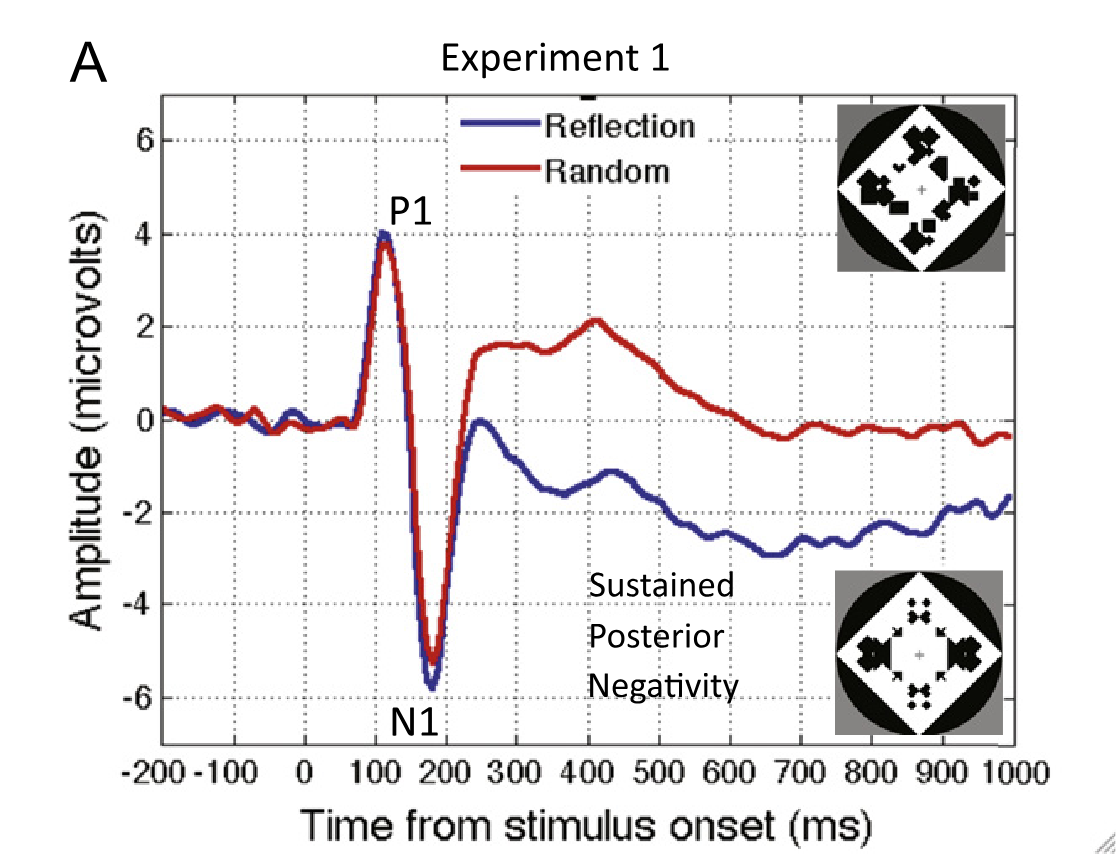
\includegraphics[width=0.8\linewidth]{assets/authors_results.png}
        \caption{Authors average results \cite{paper}}
        \label{fig:authors-results}
    \end{figure}
\end{center}

In the plot in Figure \ref{fig:authors-results}, the authors show what results they got with their processing.

Notable for us are the similar P1 peek which are relevant for tasks in visual perception. Also relevant is a reported difference in the amplitude of the N1. They mention the possibility of visual symtery detection to start even earlier as a possible reason for the appearance of this.

The continued sustained posterior negativity is part of the special symmetry perception part of their work. This will also be the part we will put the most focus on in the rest of our work. From the data, we can see the clearly different amplitudes of the levels for the reflection condition in the part between 300 and 1000 ms.
The reported amplitude clearly has a negativity associated which was named sustained posterior negativity due to its appearance.

The author further went into detail on some more info about their pipeline.

They showed a number of their cleaning step which was ICA in their canse as well as two runs of trial rejection.
Once before ICA and once after.
They reported that their ICA removed $9.42$ components on average per subject.
They got a minimum of $4$ components and a maximum of $16$ removed components throughout their $24$ subjects.

Additionally they ran a trial rejection before their ICA step with a threshold of $\pm100$ mV which removed $10.34\%$ of reflection and $9.95\%$ of random epochs. Secondly, they reran their trial rejection with a threshold of $\pm75$ mV after ICA.
This step removed another $4.06\%$ of reflection and $4.90\%$ of random trials.

The authors further looked into their recorded EOG data. This data will be relevant for our further analysis on ASR, which is why we also need to look at their results more closely.

They measured additional channels with muscle activity, including eye movement and blinks. These channels are widely called VEOG and HEOG for vertical and horizontal movements. The authors looked at these channels to confirm that there is no significant difference between the two conditions, random and regular. They stated:
\begin{quote}
    Horizontal and vertical eye electrode channels were low-pass filtered at 25 Hz
    and epoched (-1 to 1 s), but not subjected to further treatment. Mean EOG activity
    did not differ between reflection and random conditions (VEOG, $p=0.211$; HEOG,
    $p=0.185$). This provides evidence that any remaining ocular artefacts (or side effects
    of artefact correction procedures) did not selectively distort one condition.
\end{quote}

Which means they confirmed that the impact of these possible muscle artefacts did not significantly differ between the conditions.




\subsection{Our Results}\label{our-results}
Our first goal was to replicate the authors' results with our individual pipeline.
With the milestones we had throughout the semester, we had some individual sanity checks to check our progress and the effectiveness of our steps.
For example, to test our filtering, we produced a plot showing the power spectrum.
\begin{center}
    \begin{figure}[h]
        \centering
        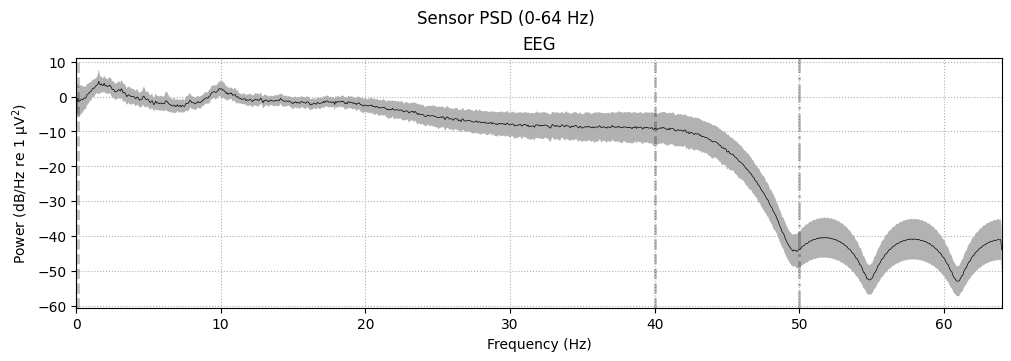
\includegraphics[width=1\linewidth]{assets/subject005/sub-005_psd.png}    
        \caption{Power spectrum for subject 005}
        \label{fig:psd005}
    \end{figure}
\end{center}

In Figure \ref{fig:psd005}, we can see that our filters removed high frequencies as intended.

Another important sanity check was a topology plot of our ICA components.

\begin{wrapfigure}[18]{R}{0.5\textwidth}
    \vspace{-1cm}\begin{center}
        \centering
        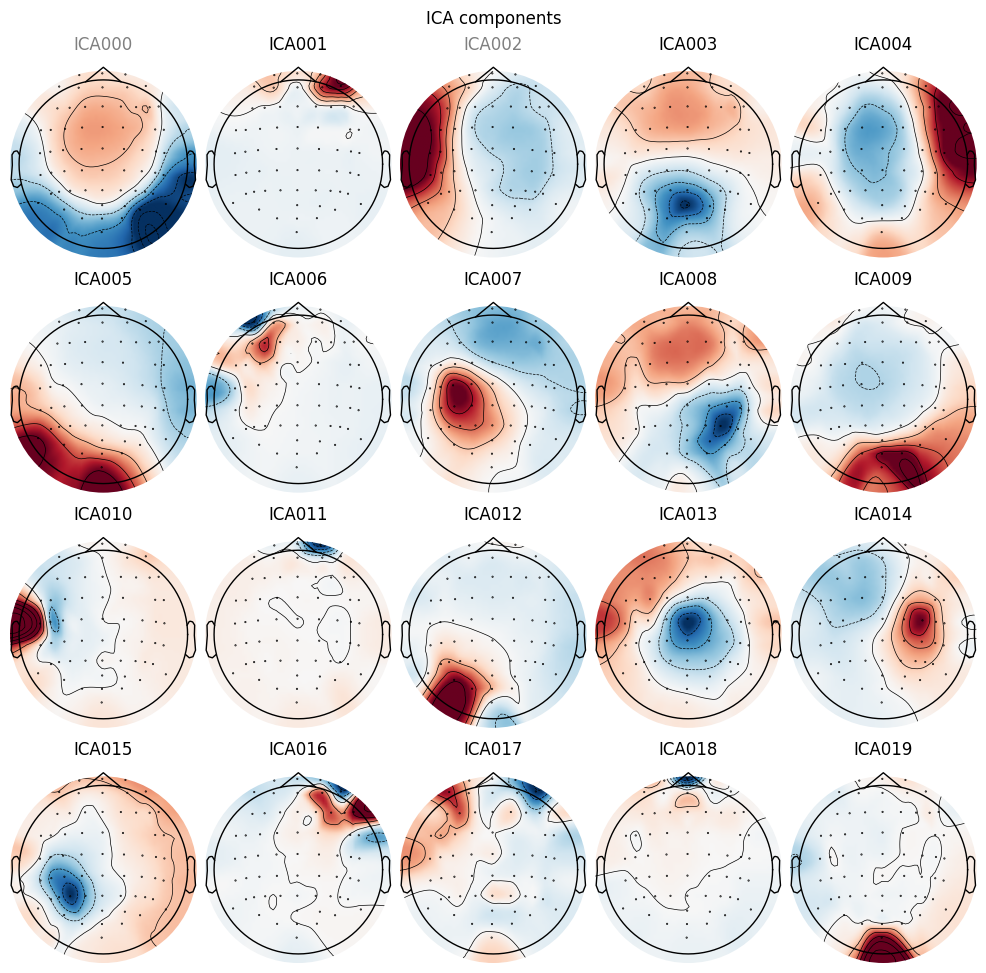
\includegraphics[width=1\linewidth]{assets/subject005/sub-005_ica.png}
        \caption{Topology of ICA components}
        \label{fig:ica-topo}
    \end{center}
\end{wrapfigure}

In Figure \ref{fig:ica-topo}. we plotted an example of our ICA components.
As discussed in the Milestone presentations, we interpret these components as not that great.
From what we have learned here, these components are quite small and spikey.
This often would show on noisy data with large peaks, which lead to these small but sharp spikes.
These spikes would show up as these components in our topology map, for example, ICA019 in Figure \ref{fig:ica-topo}.
We can not really compare our ICA to the authors' since they did not provide such a plot in their report.

When plotting these topology maps, we also ran into problems in some cases without bad-channel detection.
We assume there to be a problem with some channels, which would be marked as bad anyway.
The plot we were using and were planning on using all went through without any errors. 

These sanity checks can also be seen in our further analysis of the single steps.
On each added step, we can see the differences this is making to our data.
These steps can be looked at in Section~\ref{impact-steps}.

Our first pipeline reproduced the general morphology of the ERP waveforms reported by Makin et al.~\cite{paper}. The P1 component (around 100–130 ms) and N1 component (around $170-200$ ms) are clearly visible at PO7/PO8 in our grand average in Figure~\ref{fig:average-default}.

\begin{figure}[h]
    \centering
    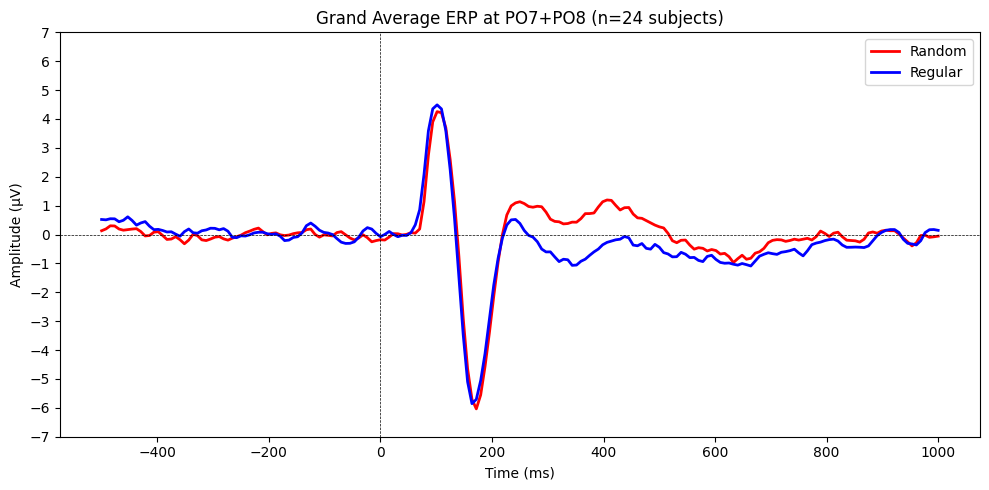
\includegraphics[width=1\linewidth]{assets/comparison/fig-average_po7po8-1-default.png}
    \caption{Pipeline with all steps enabled}
    \label{fig:average-default}
\end{figure}
The amplitudes we are getting are in a comparable range to the original study.
The overall shape of the waveforms, first a positive deflection followed by a negative deflection, matches the expected visual evoked potential pattern for pattern-onset stimuli.

However, a notable difference emerged in the sustained posterior negativity (SPN).
While the authors reported a robust SPN with a clear separation between regular and random conditions from approximately $300$ ms onward, our default pipeline shows a substantially reduced SPN.

With the statistics we got from the authors, we can also compare ICA and trial rejection.
In our standard pipeline, we removed a total of $9.9 \%$ of random and $9.43\%$ of regular trials.
This is comparable to their rejection rate of about $10 \%$ before ICA.
The authors removed another about $ 5\%$ of trials after ICA in their second trial rejection.
These numbers are quite comparable, which made us believe that the trial rejections should not be a big factor in the differences we were finding.

For the ICA component, we removed about $1.29$ components per subject, while the authors removed $9.42$ per subject.
This is a significant difference that could have an impact.
Although we ran ASR as well as ICA, which could lead to cleaner data when reaching ICA.
This would explain fewer removed components.

These differences we found here led us to further look into where these differences come from.


\section{Discussion}
When looking for a reason, our data differs from the authors results, we quickly guessed that it could have something to do with ASR.
Since this is the most drastic change in our pipelines, we assumed this to be a good candidate for a first inspection.

When writing the second config for our pipeline, we just removed ASR and plotted everything we needed to compare again.
\begin{figure}[h]
    \centering
    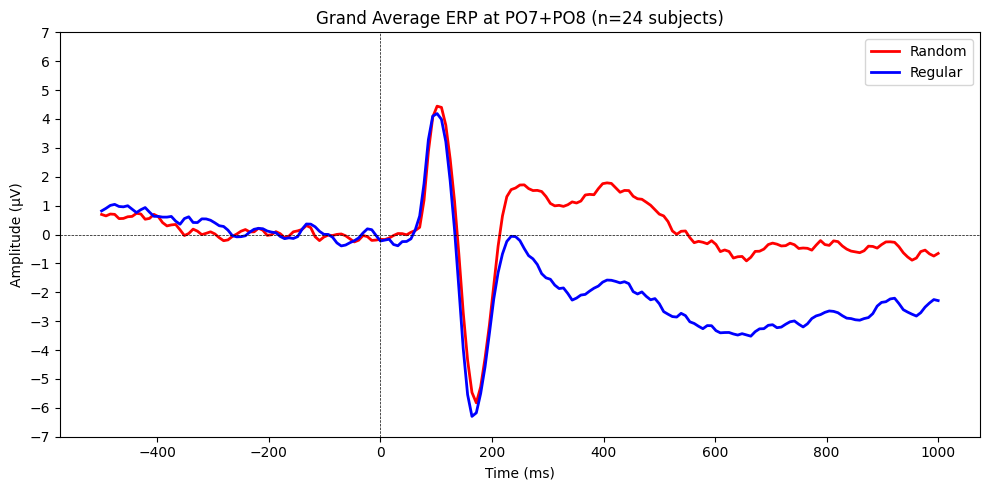
\includegraphics[width=1\linewidth]{assets/comparison/fig-average_po7po8-2-noasr.png}
    \caption{Results without ASR}
    \label{fig:average-noasr}
\end{figure}

In our final plot in Figure~\ref{fig:average-noasr}, we can clearly see that the missing SPN of our original results is now present.
This quickly led us to the reason our results differed.

For the statistics on this run, we can see that we removed a little more trials with $15.1\%$ for random and $14.69\%$ for regular trials. This change can be expected since ASR had cleaned the data more. So, without this additional cleaning, there can be more rejected trials. We also found only $0.92$ ICA components pre-subject where removed. This does not align with our expectations. We assumed this would be higher because ICA had to remove more noise because ASR didn't this time. We can not really tell why this is the way it is.

We now want to find out why ASR changes the results in such a drastic way. From the definition and our understanding, ASR detects and removes transient, high-amplitude/artifactual activity. All these findings raised the question of whether ASR, rather than improving data quality, was removing signal components relevant to the ERP effects we aimed to replicate.

This concern is not unique to our work. \cite{leftalone} compared various automated preprocessing strategies for EEG data and found that minimal preprocessing, or even no preprocessing beyond basic filtering, often produced comparable or better results than complex automated pipelines. Their analysis suggests that aggressive artifact correction methods can inadvertently distort the very signals researchers aim to study, particularly when the correction method cannot distinguish between artifact and neural activity that happen to share temporal or spatial characteristics.



\subsection{Cause of ASR problems}\label{asr-problems}
To find out why ASR removes the differences, we came up with two ideas. We first want to look at the differences in the parameters for the cutoff in ASR. We wanted to try modifying this parameter to find out if ours was too aggressive and removed actual good data.

Secondly, we wanted to find out if blinks and the resulting muscle artefacts are the cause. Blinks produce large transient deflections that ASR would identify as deviating from its clean reference subspace. Since our experiment involves visual stimuli presented for three seconds per trial, blinks are expected to occur frequently during epochs and affect both conditions.  As previously stated, the authors looked into the problem of blinks and eye movements as well. They looked at the difference between random and regular conditions and how EOG differed.  They didn't find statistical differences in their analysis \cite{paper}.

Their check only confirms that blinks were balanced across conditions; it does not address whether blink-related activity, present equally in both conditions, might contribute to the overall ERP morphology that ASR then removes. To investigate this, we took a two-pronged approach: first, we implemented automatic blink detection on the EOG channels to classify each epoch as containing a blink or not. Second, we compared the grand average ERPs separately for blink and non-blink epochs, both with and without ASR, to determine whether blinks could explain the observed differences.

\subsection{Differing ASR}
When comparing our pipeline results with and without ASR, we observed that the sustained posterior negativity, the key ERP marker of symmetry perception, was substantially reduced when ASR was enabled. This difference was consistent across subjects and clearly visible in the grand average (compare Figures \ref{fig:average-default} and \ref{fig:average-noasr}). This finding was initially unexpected, as ASR is designed to remove transient artifacts while preserving the underlying signal. We hypothesized that ASR might be removing signal components that co-occur with eye blinks, which are transient high-amplitude events that ASR would treat as artifacts. Since blinks affect frontal channels most strongly but propagate to posterior sites through volume conduction, their removal by ASR could alter the ERP waveform at PO7/PO8. To test this hypothesis, we implemented automatic blink detection using the EOG channels and analyzed epochs with and without detected blinks separately.


\subsubsection{Different ASR parameters}\label{asr-parameters}
We tested different cutoff values for ASR. In the default pipeline (see Figure \ref{fig:average-default}), ASR's cutoff value was set to $10$. Lower values result in a more aggressive cutoff behavior, and higher values are more relaxed. We tested cutoff values of $20$ (Figure \ref{fig:comparison_asr20}) and $5$ (Figure \ref{fig:comparison_asr5}). As we can see, the more aggressive cutoff produces slightly smaller absolute values than the more relaxed version. However, the impact appears to be minor.

\begin{figure}[h]
    \centering
    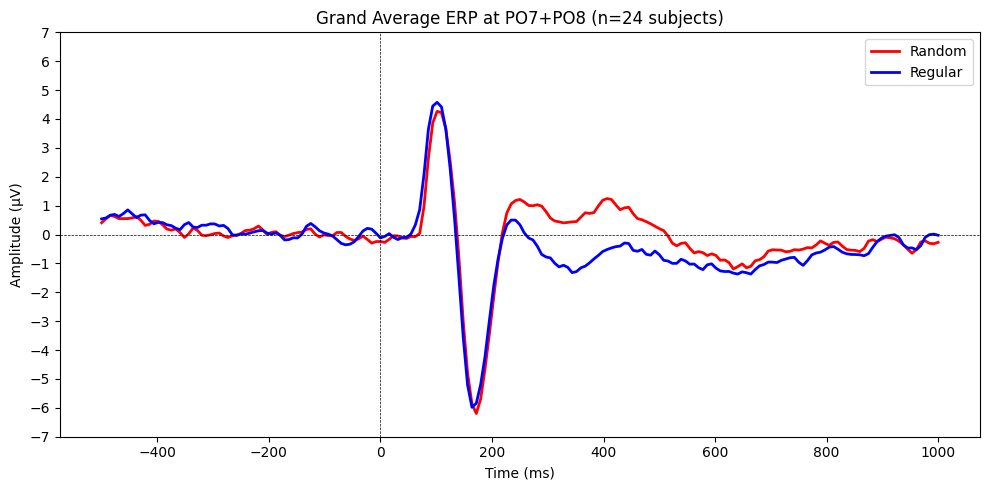
\includegraphics[width=1\linewidth]{assets/comparison/fig-average_po7po8-8-filterbadchannelrereferencingasr20.png}
    \caption{Pipeline with ASR cutoff set to 20}
    \label{fig:comparison_asr20}
\end{figure}
\vspace{-0.5cm}\begin{figure}[h]
    \centering
    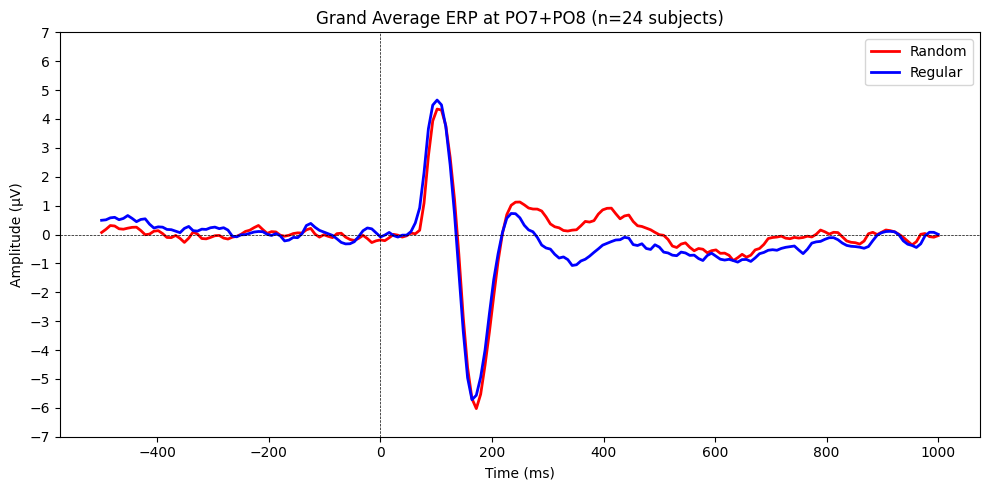
\includegraphics[width=1\linewidth]{assets/comparison/fig-average_po7po8-9-filterbadchannelrereferencingasr5.png}
    \caption{Pipeline with ASR cutoff set to 5}
    \label{fig:comparison_asr5}
\end{figure}


\subsection{Blink detection}
To determine if blinks and/or eye movements are the cause of anything we are observing, we have to identify them in the EEG data first.
We had to find out for ourselves which of the EXG-channels are the EOG-channels, since the authors did not specify the context of each individual EXG-channel in their report.

From plotting and looking at all available EXG-channels, we found EXG5 and EXG6 to most likely be the EOG-channels we are looking for. With a visual inspection of the plot, with an example excerpt in Figure \ref{fig:eogchannels}, we were convinced that these bumps in the channels are most likely blinks.
With the knowledge we gained in the lecture and from everything we've seen about blinks so far, this was the most fitting and likely case to us.
Therefore, we used these channels as our EOG data in the following analysis.

\begin{figure}[h]
    \centering
    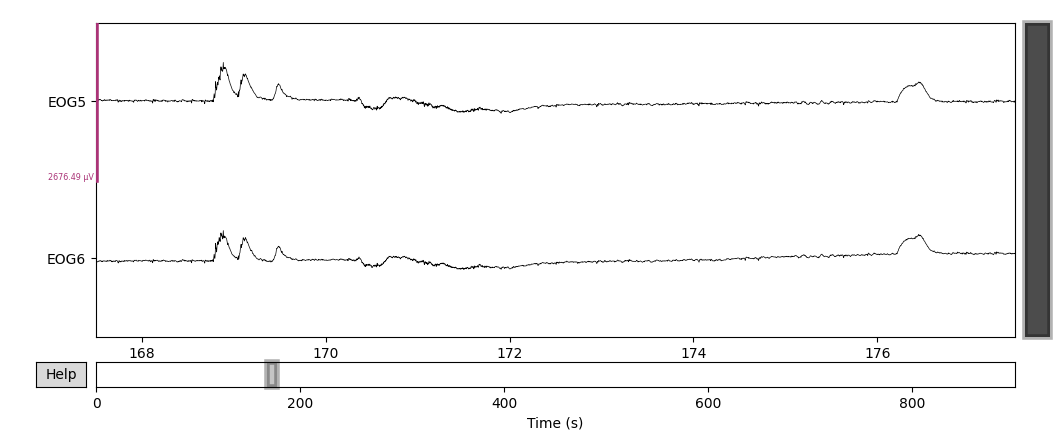
\includegraphics[width=1\linewidth]{assets/blink_detection/EOG5_6_channels_example.png}
    \caption{EOG5 and EOG6 as presumable EOG channels}
    \label{fig:eogchannels}
\end{figure}

We assume that these bumps, which we can see on the plot in Figure \ref{fig:eogchannels} are indeed blinks, and we want to identify these on the whole data set. To continue the route we went on from the beginning to do everything as automatically as possible, we wanted to do this blink-detection automatically as well. From looking online at other instances of similar tasks and confronting AI as well, we came up with an algorithm to detect these blinks on the given data.

This detection is based on a threshold, which itself is based on the mean and amplitudes of these channels. The idea is that we identify larger shifts in voltage with a threshold and mark the whole area of blinks as a whole. That way, we do not mark rising and falling edges as individual blinks.

Because this was mostly taken from other implementations and AI worked on the code, we had to look into these results to confirm that we actually compute what we want. For this check, we plotted the given EOG channels as well as the channels PO7 and PO8. We then ran the algorithm for blink-detection and marked each area where a blink was detected.

For plotting, we choose to plot only data around epochs since this is the data we will be inspecting further.

In Figures \ref{fig:epoch_blink}, \ref{fig:epoch_partialblink} and \ref{fig:epoch_noblink}, we can see example epochs with, with partial or without blinks.

\begin{figure}[h]
    \centering
    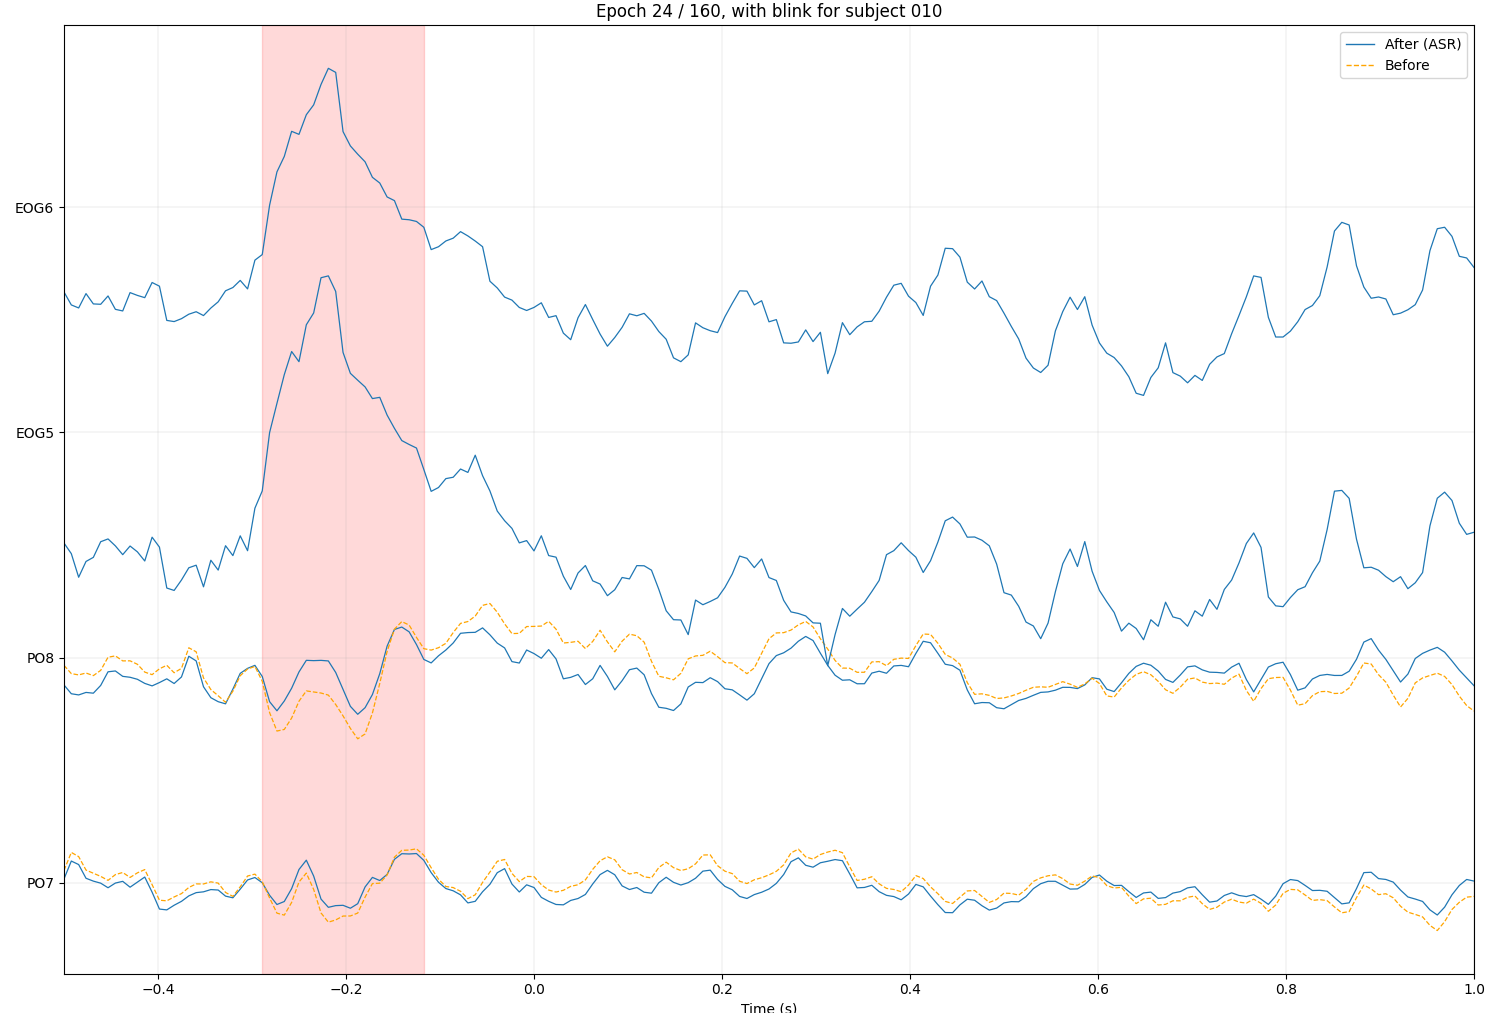
\includegraphics[width=1\linewidth]{assets/blink_detection/blink_asr_diff.png}
    \caption{Epoch with blink}
    \label{fig:epoch_blink}
\end{figure}
\begin{figure}[h]
    \centering
    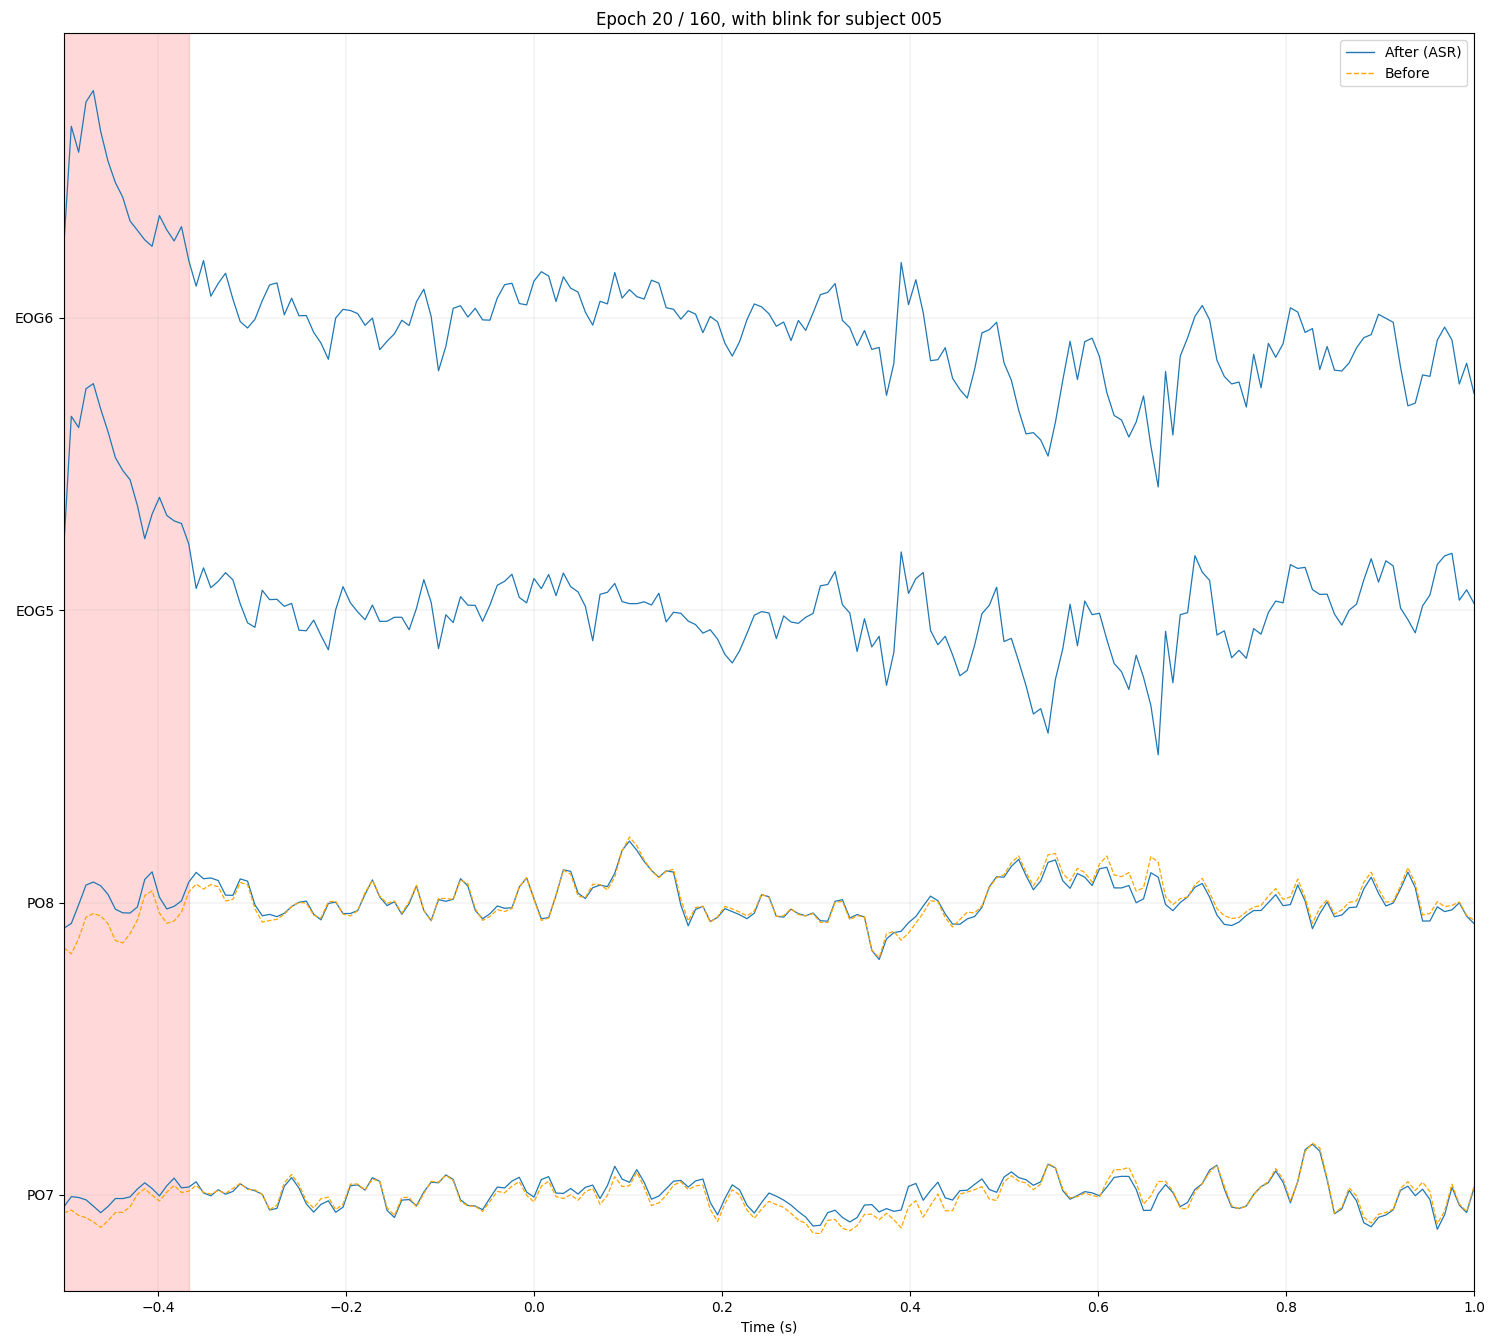
\includegraphics[width=1\linewidth]{assets/blink_detection/blink_example_asr_vs_nonasr.png}
    \caption{Epoch with partial blink}
    \label{fig:epoch_partialblink}
\end{figure}
\begin{figure}[h]
    \centering
    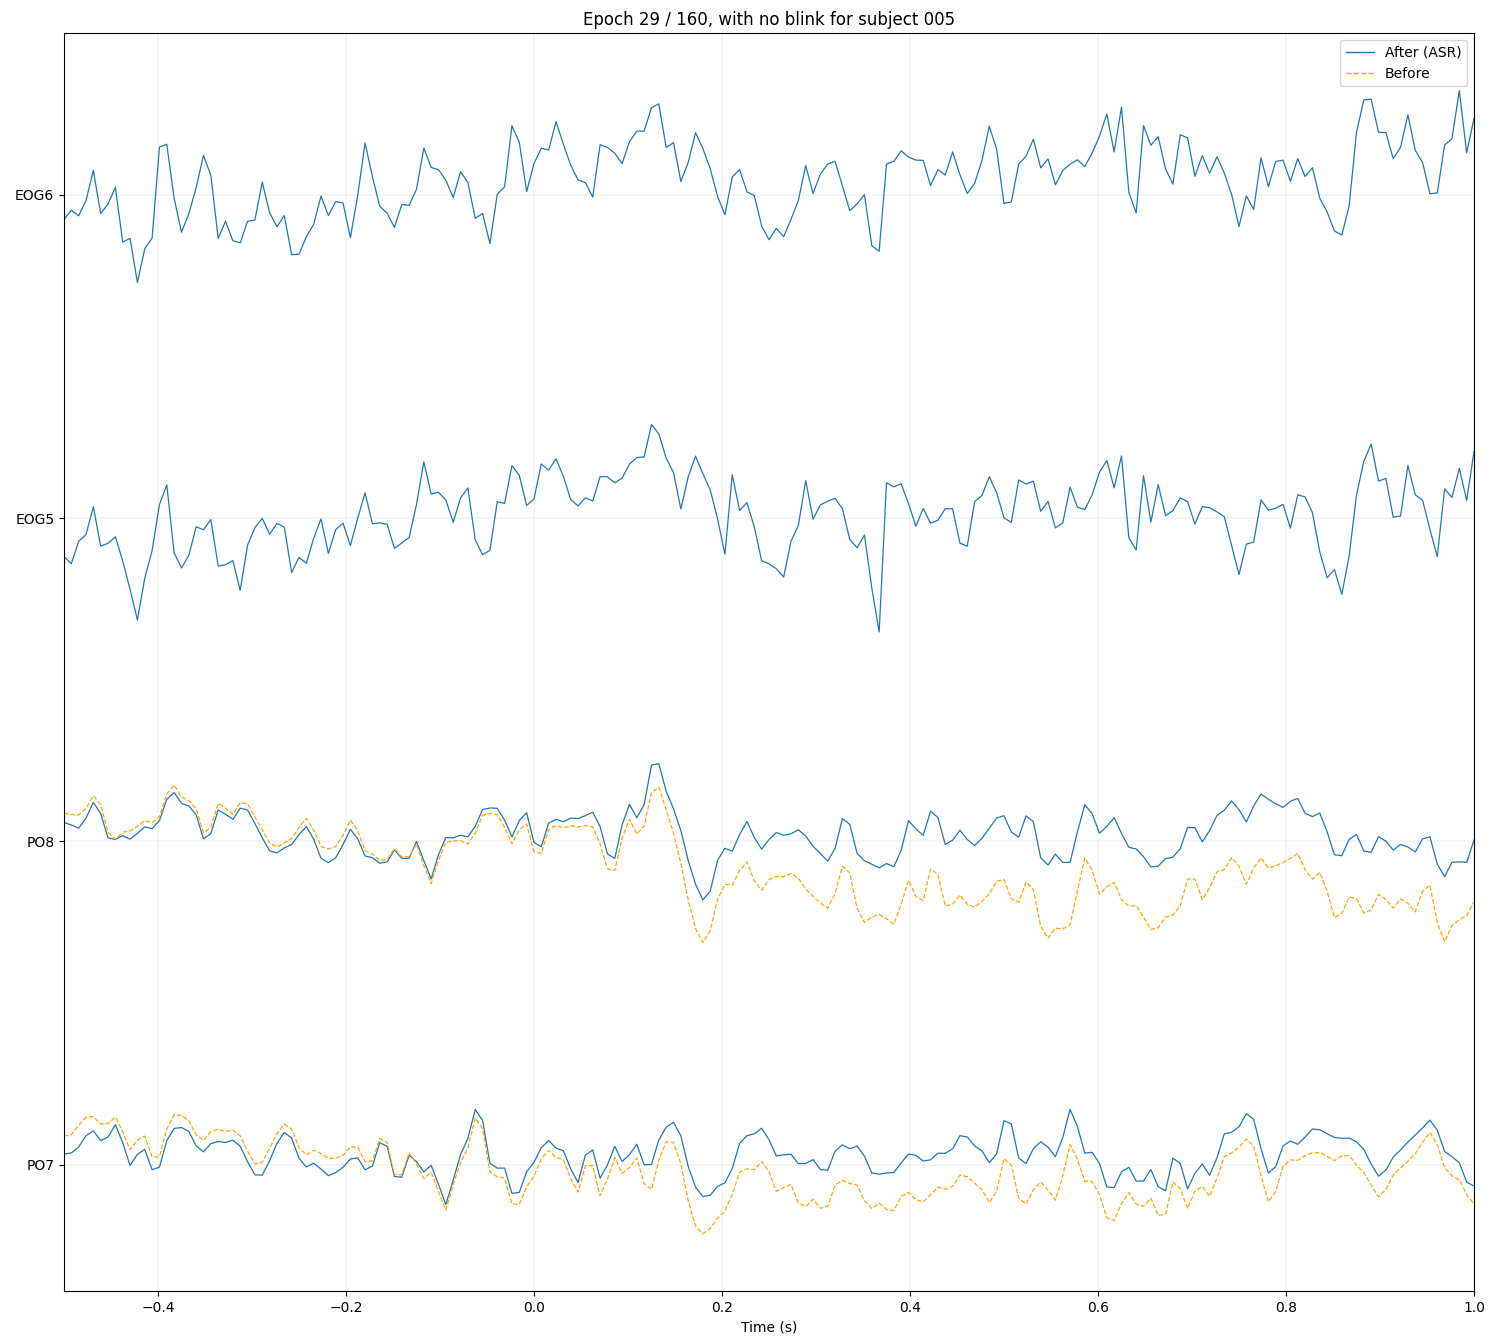
\includegraphics[width=1\linewidth]{assets/blink_detection/blink_example2_asr_vs_nonasr.png}
    \caption{Epoch with no blink}
    \label{fig:epoch_noblink}
\end{figure}

When looking at lots of these plots, we found this algorithm to work well enough for our cases.
We are also not sure how we would easily improve the detection of blinks further here.

With this automatic detection of blinks, we could further dig into the impact of these.



\subsubsection{Difference with blinks}
After we identified blinks from the provided data, we now wanted to see if these blinks indicate some kind of difference when running ASR at all. For this, we first modified the plots from before to also include the channels PO7 and PO8 after ASR was enabled in the pipeline. These can already be seen in the Figures \ref{fig:epoch_blink}, \ref{fig:epoch_partialblink} and \ref{fig:epoch_noblink} from before. Here we plotted the pipeline run with and without ASR in relation to our blink detection.

In these examples, we can see that on large offsets in the EOG channels, we generally can also see a bigger difference in the EEG channels with ASR. But we can also see in Figure \ref{fig:epoch_noblink} that there are differences with no blink detected.

This led us to believe that blinks could be an influence in the differences we observe with ASR, but probably are not the only ones.


\subsubsection{Impact on average}
With the now implemented blink-detection and the differences in ASR/non-ASR runs, we wanted to look into the differences in a grand average scenario again. Looking into specific epochs and only specific subjects is not in any way meaningful for the whole picture, our pipeline, and the authors looked at.

We came up with the idea to run this pipeline on each subject we have and split all epochs we have into two buckets based on the condition of a detected blink or not. With this data, we hoped to maybe see a difference when plotting the grand average as usual, but separated by blinks.

For this, we split all epochs on the condition blink and luckily got a good enough sample size for both. With all 24 subjects, we ended up with 1341 epochs with a detected blink and 2499 epochs without a blink. This was a good enough split for us to be still quite confident in the sample size for the blink-epochs. We felt like 1341 is still a decent amount to be looking further into this, because a too small sample set would probably lead to way worse results and vastly different plots because of statistical relevance.

\begin{figure}[h]
    \centering
    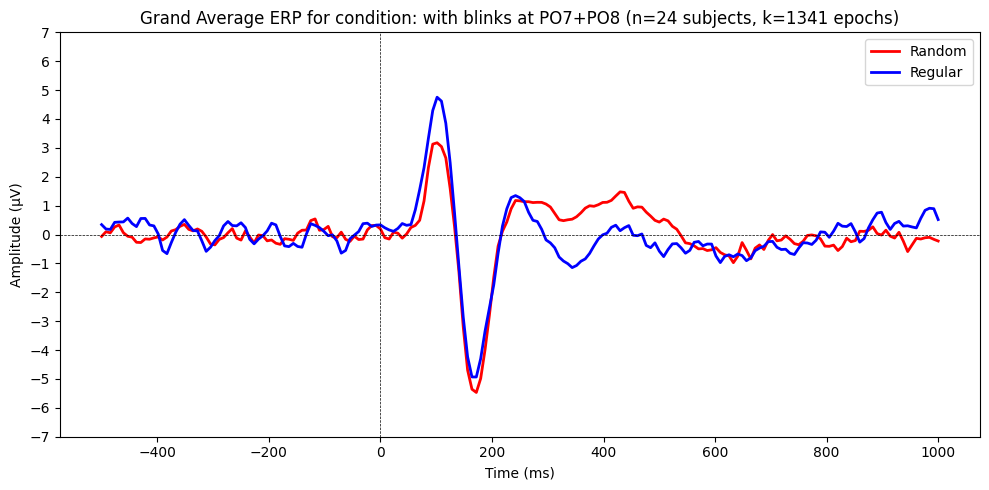
\includegraphics[width=0.9\linewidth]{assets/blink_detection/fig-average_po7po8_ASR_with_blinks.png}
    \caption{Pipeline with ASR and only blink epochs}
    \label{fig:average_asr_blink}
\end{figure}
\begin{figure}[!h]
    \centering
    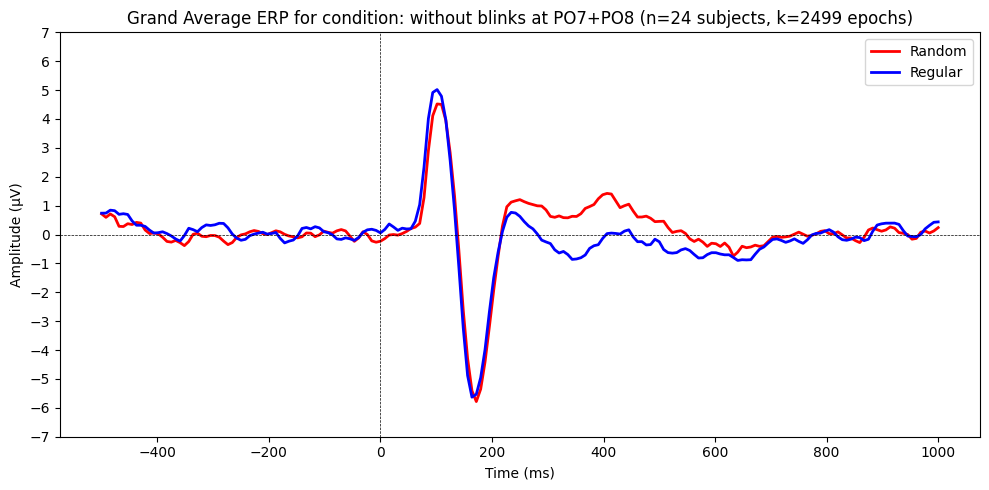
\includegraphics[width=0.9\linewidth]{assets/blink_detection/fig-average_po7po8_ASR_without_blinks.png}
    \caption{Pipeline with ASR and only noblink epochs}
    \label{fig:average_asr_noblink}
\end{figure}

The Figures \ref{fig:average_asr_blink} and \ref{fig:average_asr_noblink} show the normal pipeline(with ASR) and our splitting of the blink condition. In these plots, we can see no real difference in the sustained posterior negativity. Interestingly, we are seeing a much smaller P1 with blinks on random patterns. We can not explain why this might be the case. We assume that this might be an artifact from using fewer epochs (only 1341), but we are not sure of any other possible causes for this.

To continue, we also plotted the results for the pipeline with ASR disabled in Figures \ref{fig:average_blink} and \ref{fig:average_noblink}.
In these plots, we can again observe a smaller P1 peak for epochs with blinks. Again, we are not fully sure of how this came about. We still assume this might be because of smaller epoch sizes or something we could not identify.
\begin{figure}[!h]
    \centering
    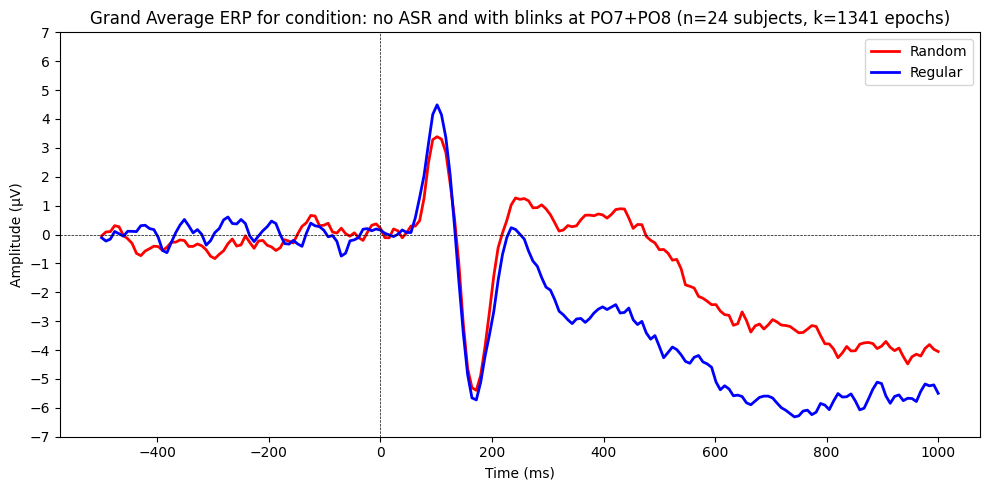
\includegraphics[width=0.9\linewidth]{assets/blink_detection/fig-average_po7po8_with_blinks.png}
    \caption{Pipeline without ASR and only blink epochs}
    \label{fig:average_blink}
\end{figure}
\begin{figure}[!h]
    \centering
    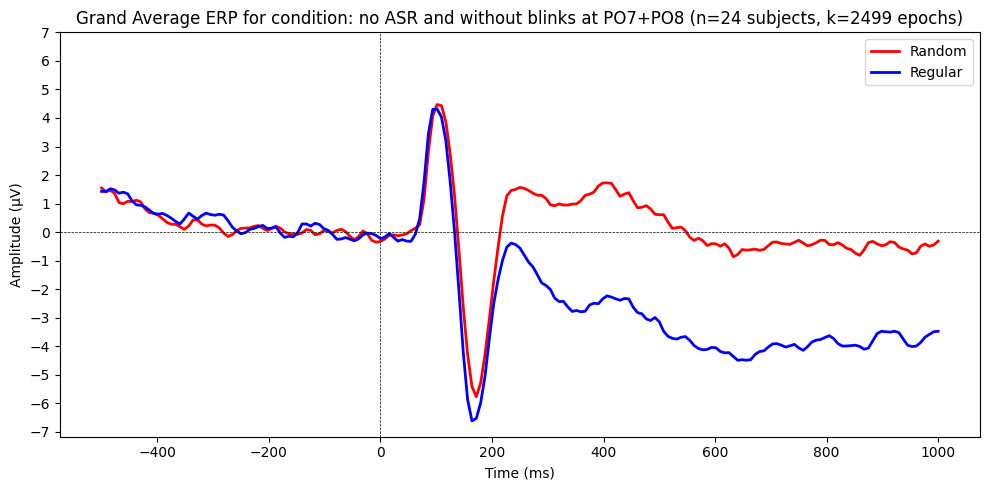
\includegraphics[width=0.9\linewidth]{assets/blink_detection/fig-average_po7po8_without_blinks.png}
    \caption{Pipeline without ASR and only noblink epochs}
    \label{fig:average_noblink}
\end{figure}

But more interestingly, we can see quite a significant difference in these two plots. We can see that there is a difference between the levels of amplitude between the conditions of random/regular in both cases. We can also see a much more downshifted activity towards the end of blink epochs in Figure \ref{fig:average_blink}.

Both of these plots show indications of the difference in the sustained posterior negativity that we found in our original comparison between ASR and non-ASR runs. The fact that there is a way larger offset in blink epochs in comparison to non-blink epochs also suggests that there is a statistically relevant difference with present blinks in an epoch.


\subsubsection{Discussion of blink detection}
Our interpretation of the results we have seen about our deep-dive into blink-detection and the impact of ASR in that case, is that these might actually be one of the reasons the original results differed with ASR.

As stated before, we can also see a significant difference between Figure \ref{fig:average_asr_noblink} and Figure \ref{fig:average_blink}. This should be data, where no blinks are present, and we can still observe a significant difference in the sustained posterior negativity. We assume that there are other hidden artifacts, which ASR is removing, that we did not consider here.
But we can also state that the difference in blink epochs is also significant.

Therefore, we claim that the blinks we detected are one of the possible causes of the difference between ASR and non-ASR runs.


\subsection{Impact of Steps}\label{impact-steps}
To analyze the impact of each preprocessing step, we ran nine pipeline configurations that progressively add steps (see Table \ref{tab:configs}). For each configuration, we generated grand average ERPs, power spectral density plots, butterfly plots, and topographic maps for a certain subject. The choice of the subject was arbitrary and other subjects gave similar plots. In the following, we compare successive configurations to isolate each step's contribution.

\begin{table}[h]
    \centering
    \begin{tabular}{l|l}
        ID & Description  \\\hline
        1 & Default (every step of our pipeline enabled, see Section \ref{pipeline}) \\\hline
        2 & No ASR (All other steps are enabled) \\\hline
        3 & Nothing (only the mandatory steps downsampling and epoching are enabled) \\\hline
        4 & only filter (added filtering) \\\hline
        5 & filtering and badchannel detection \\\hline
        6 & filtering, badchannel detection and rereferencing \\\hline
        7 & filtering, badchannel detection, refreferencing and asr (no ICA) \\\hline
        8 & Same as 7, asr cutoff value set to 20 \\\hline
        9 & Same as 7, asr cutoff value set to 5
    \end{tabular}
    \caption{Configurations overview}
    \label{tab:configs}
\end{table}

\subsubsection{Baseline - Only loading and downsampling}
Our starting point was the pipeline with the two mandatory steps, loading and downsampling from 512 Hz to 128 Hz enabled. This represents the rawest view of the data our pipeline can produce. The power spectral density plot (see Figure \ref{fig:sub005-psd-3}) for this configuration shows the expected $\frac{1}{f}$ spectral slope with peaks around 10 Hz and 50 Hz. The latter is typically produced by power line interferences. The gray shaing in the psd represents the spread across channels. The wide spread indicates large inter-channel variability probably due to bad channels.

\begin{figure}[h]
    \centering
    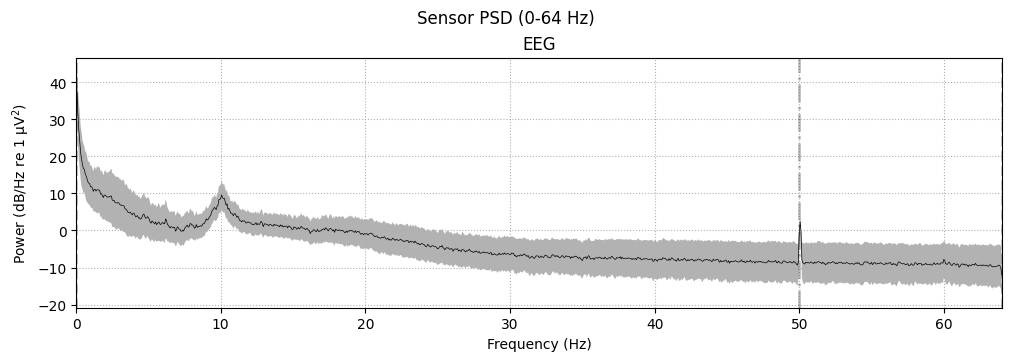
\includegraphics[width=0.8\linewidth]{assets/subject005/sub-005_psd-3-nothing.png}
    \caption{Subject 005 - Config 3 PSD}
    \label{fig:sub005-psd-3}
\end{figure}
\begin{figure}[h]
    \centering
    \hspace{-2cm}\begin{minipage}{.59\textwidth}
        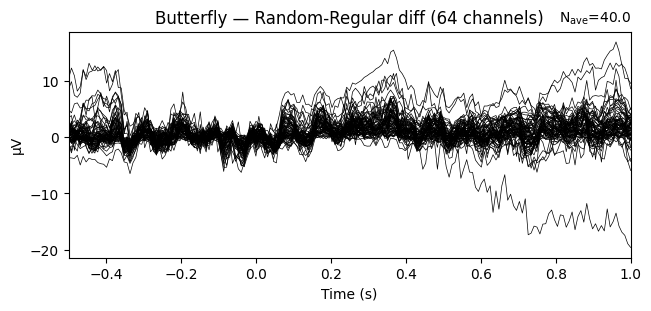
\includegraphics[width=1.2\linewidth]{assets/subject005/sub-005_butterfly_combined-3-nothing.png}
        \captionof{figure}{Subject 005 - Config 3 Butterfly}
        \label{fig:sub005-butterfly-3}
    \end{minipage}\hspace{1.5cm}
    \begin{minipage}{.4\textwidth}
        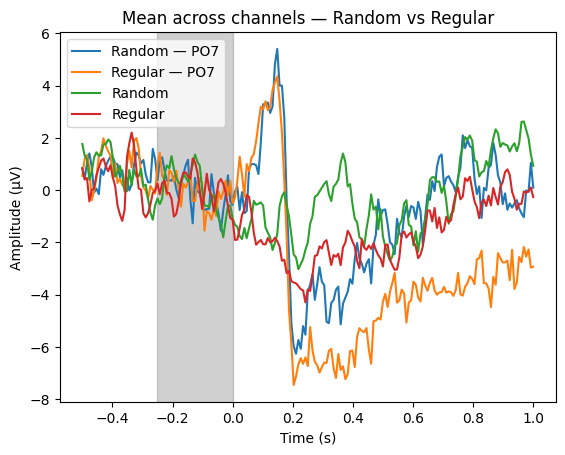
\includegraphics[width=1.2\linewidth]{assets/subject005/sub-005_all_channel_erp-3-nothing.png}
        \captionof{figure}{Subject 005 - Config 3 All Channels ERP}
        \label{fig:sub005-all-erp-3}
    \end{minipage}
\end{figure}

The butterfly plot (Figure \ref{fig:sub005-butterfly-3}) shows individual channel traces spanning approximately $\pm 15\mu V$, with several extreme outlier channels reaching beyond $\pm 20 \mu V$. High-frequency jitter is visible throughout, reflecting the unfiltered muscle and environmental noise. Despite this, the all-channel ERP at PO7 (Figure \ref{fig:sub005-all-erp-3}) already shows a recognizable P1 and N1 pattern, demonstrating that the evoked response is strong enough to show even from completely unprocessed data when averaged across all trials. The global mean across all channels (green and red lines) hovers around zero but with substantial noise, and a visible separation between random and regular conditions is present but obscured by the noise floor. This baseline establishes both what the raw data looks like and how much of the ERP structure is inherently present in the signal before any cleaning.

\subsubsection{Filtering}
The psd plot clearly shows the effect of the filtering step: Config 3 has a significant spike at 50 Hz from the power grid noise and substantial power above 40 Hz which both are removed in config 4 (see Figure \ref{fig:sub005-psd-4}). The low-pass creates a sharp rolloff at 40 Hz, and the notch filter eliminates the 50 Hz peak cleanly. The all-channel ERP (Figure \ref{fig:sub005-all-erp-3}) plot shows that the general ERP morphology (P1, N1) is already visible even without filtering, but the waveforms in config 4 (Figure \ref{fig:sub005-all-erp-4}) are noticeably smoother.

\begin{figure}[h]
    \centering
    \hspace{-2cm}\begin{minipage}{.59\textwidth}
        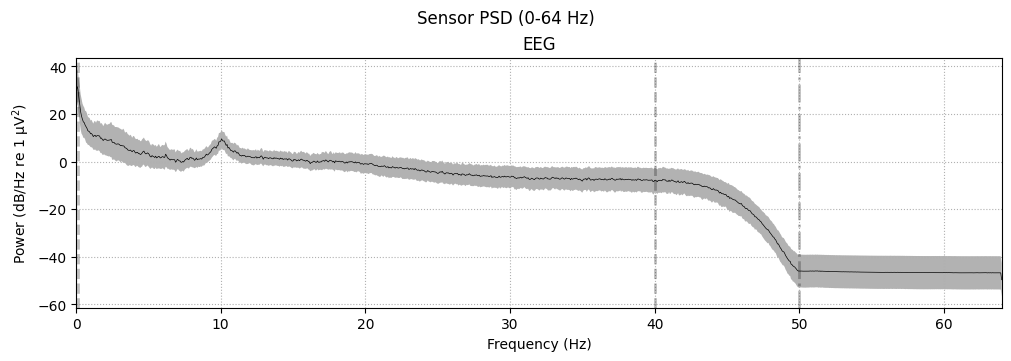
\includegraphics[width=1.2\linewidth]{assets/subject005/sub-005_psd-4-onlyfilter.png}
        \captionof{figure}{Subject 005 - Config 4 PSD}
        \label{fig:sub005-psd-4}
    \end{minipage}\hspace{1.8cm}
    \begin{minipage}{.4\textwidth}
        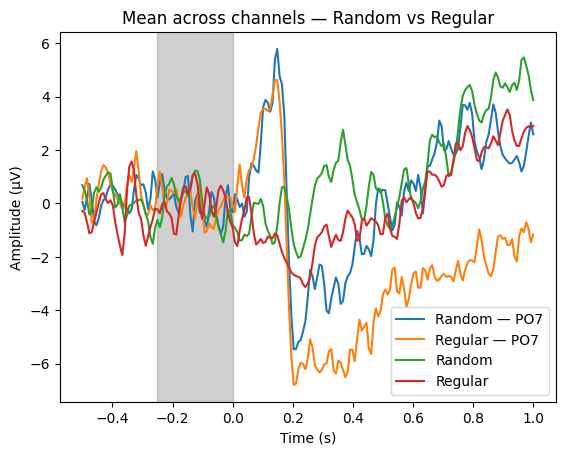
\includegraphics[width=1.2\linewidth]{assets/subject005/sub-005_all_channel_erp-4-onlyfilter.png}
        \captionof{figure}{Subject 005 - Config 4 All Channels ERP}
        \label{fig:sub005-all-erp-4}
    \end{minipage}
\end{figure}

\subsubsection{Bad Channel Detection}
 The butterfly plot reveals this step's effect most clearly: config 4 has 64 channels with several extreme outlier traces reaching $\pm 20 \mu V$, while config 5 drops to 61 channels (three channels marked bad for this subject) and the outlier traces disappear (Figure \ref{fig:sub005-butterfly-5}), reducing the range to approximately $\pm 15 \mu V$. The all-channel ERP (Figure \ref{fig:sub005-all-erp-5}) shows slightly reduced peak amplitudes, consistent with removing channels that were pulling the average toward extreme values.
\begin{figure}[h]
    \centering
    \hspace{-2cm}\begin{minipage}{.59\textwidth}
        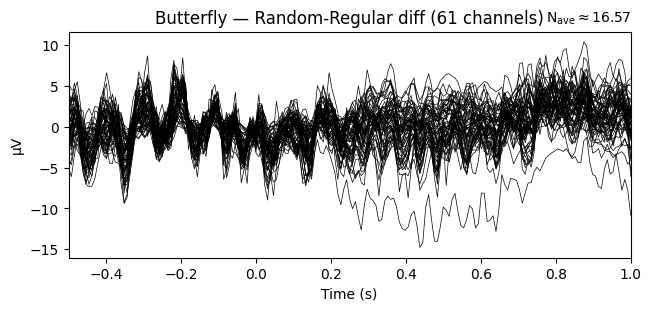
\includegraphics[width=1.2\linewidth]{assets/subject005/sub-005_butterfly_combined-5-filderbadchannel.png}
        \captionof{figure}{Subject 005 - Config 5 Butterfly}
        \label{fig:sub005-butterfly-5}
    \end{minipage}\hspace{1.5cm}
    \begin{minipage}{.4\textwidth}
        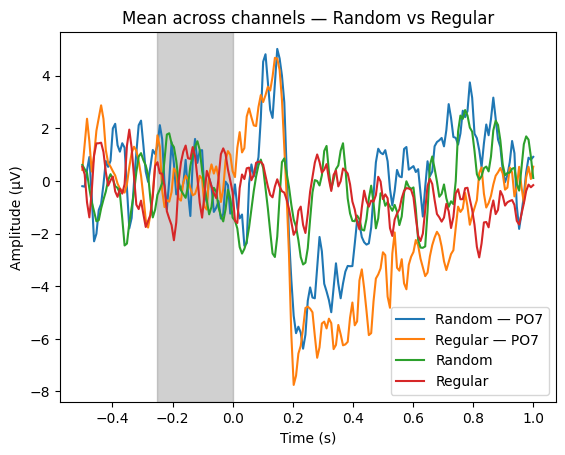
\includegraphics[width=1.2\linewidth]{assets/subject005/sub-005_all_channel_erp-5-filderbadchannel.png}
        \captionof{figure}{Subject 005 - Config 5 All Channels ERP}
        \label{fig:sub005-all-erp-5}
    \end{minipage}
\end{figure}


\subsubsection{Rereferencing}
The psd (Figure \ref{fig:sub005-psd-6}) shows a notable reduction in inter-channel variance: the gray shading (representing spread across channels) narrows substantially after average re-referencing, meaning channels become more similar to each other. The biggest change is in the all-channel ERP (Figure \ref{fig:sub005-all-erp-6}): the global mean across all channels (green and red lines) collapses to approximately zero after re-referencing. This is expected as average referencing makes the instantaneous mean across channels zero by definition. The PO7 traces retain their ERP structure but now represent deviations from the scalp average rather than from the original recording reference, which is the physically more meaningful quantity.
\begin{figure}[h]
    \centering
    \hspace{-2cm}\begin{minipage}{.59\textwidth}
        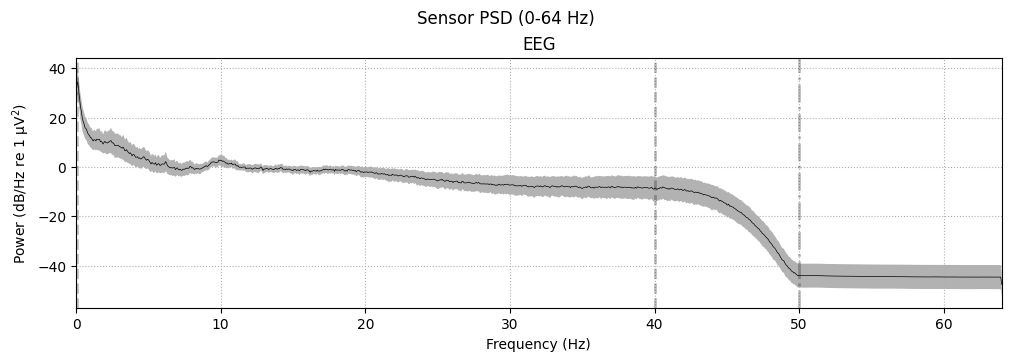
\includegraphics[width=1.2\linewidth]{assets/subject005/sub-005_psd-6-filterbadchannelrereferencing.png}
        \captionof{figure}{Subject 005 - Config 6 PSD}
        \label{fig:sub005-psd-6}
    \end{minipage}\hspace{1.8cm}
    \begin{minipage}{.4\textwidth}
        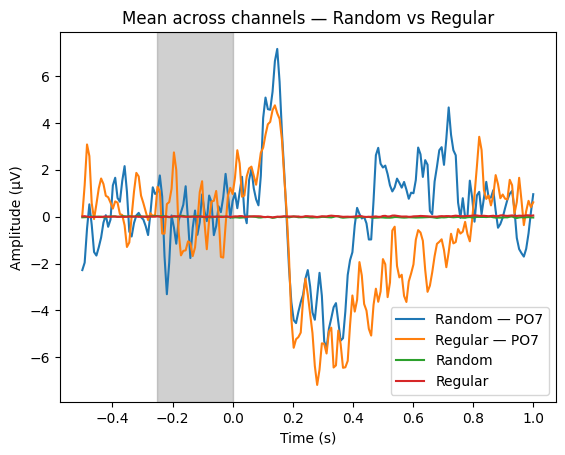
\includegraphics[width=1.2\linewidth]{assets/subject005/sub-005_all_channel_erp-6-filderbadchannelrereferencing.png}
        \captionof{figure}{Subject 005 - Config 6 All Channels ERP}
        \label{fig:sub005-all-erp-6}
    \end{minipage}
\end{figure}

\subsubsection{ASR}
ASR produces the most dramatic signal compression visible in the plots. The psd (Figure \ref{fig:sub005-psd-7}) drops from a maximum of approximately 40 dB/Hz to about 10 dB/Hz, indicating that ASR is removing a large portion of the signal's total power. The butterfly plot confirms this (Figure \ref{fig:sub005-psd-7}): the trace spread shrinks from $\pm 10\mu V$ to approximately $\pm 4 \mu V$ (Figure \ref{fig:sub005-butterfly-7}), a compression by more than a factor of two. The all-channel ERP at PO7 looks similar in shape between configs 6 and 7 for a single subject, but the grand average across all subjects (discussed in Section \ref{asr-parameters}) reveals that this compression attenuates the sustained posterior negativity that distinguishes conditions.
\begin{figure}[h]
    \centering
    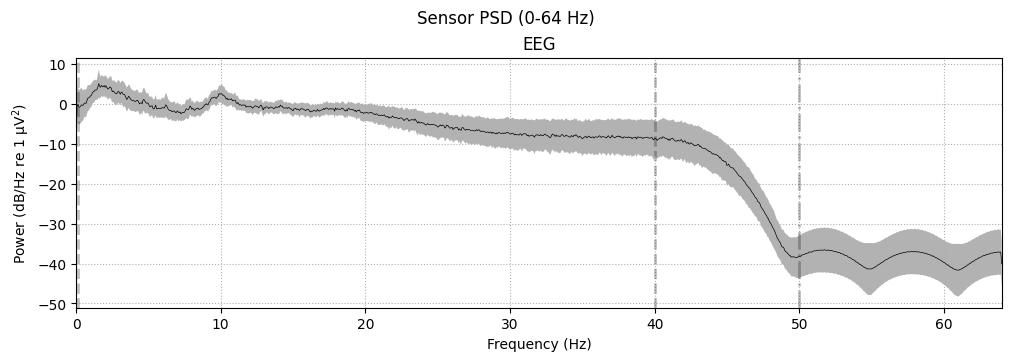
\includegraphics[width=0.8\linewidth]{assets/subject005/sub-005_psd-7-filterbadchannelrereferencingasr.png}
    \caption{Subject 005 - Config 7 PSD}
    \label{fig:sub005-psd-7}
\end{figure}
\begin{figure}[h]
    \centering
    \hspace{-2cm}\begin{minipage}{.59\textwidth}
        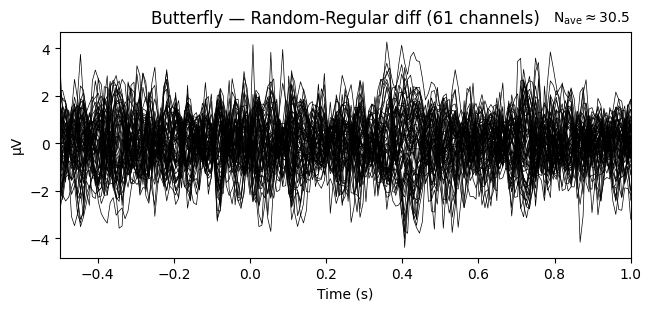
\includegraphics[width=1.2\linewidth]{assets/subject005/sub-005_butterfly_combined-7-filderbadchannelrereferencingasr.png}
        \captionof{figure}{Subject 005 - Config 7 Butterfly}
        \label{fig:sub005-butterfly-7}
    \end{minipage}\hspace{1.5cm}
    \begin{minipage}{.4\textwidth}
        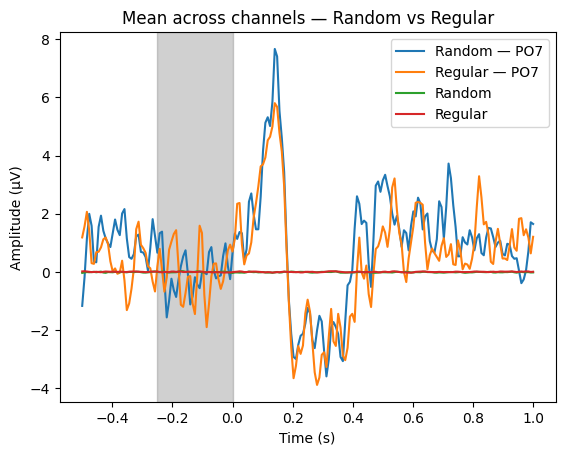
\includegraphics[width=1.2\linewidth]{assets/subject005/sub-005_all_channel_erp-7-filderbadchannelrereferencingasr.png}
        \captionof{figure}{Subject 005 - Config 7 All Channels ERP}
        \label{fig:sub005-all-erp-7}
    \end{minipage}
\end{figure}


\subsubsection{Full pipeline: ASR vs no ASR}
Comparing the full pipeline with (Figure \ref{fig:sub005-all-erp-1}) and without ASR (Figure \ref{fig:sub005-all-erp-2}; both including ICA, interpolation, and trial rejection), the single-subject all-channel ERP at PO7 shows that config 2 (no ASR) has larger negative deflections in the $300-1000$ ms window compared to config 1. While single-subject plots are noisy, this is consistent with the grand average finding that ASR attenuates the SPN. 

\begin{figure}[h]
    \centering
    \hspace{-2cm}\begin{minipage}{.49\textwidth}
        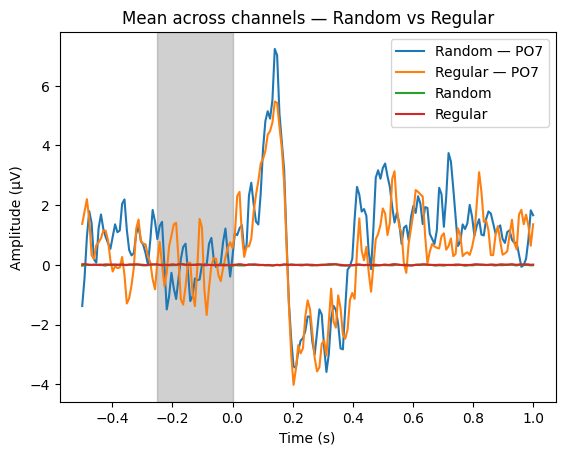
\includegraphics[width=1.1\linewidth]{assets/subject005/sub-005_all_channel_erp-1-default.png}
        \captionof{figure}{Subject 005 - Config 1 All Channels ERP (with ASR)}
        \label{fig:sub005-all-erp-1}
    \end{minipage}\hspace{1cm}
    \begin{minipage}{.49\textwidth}
        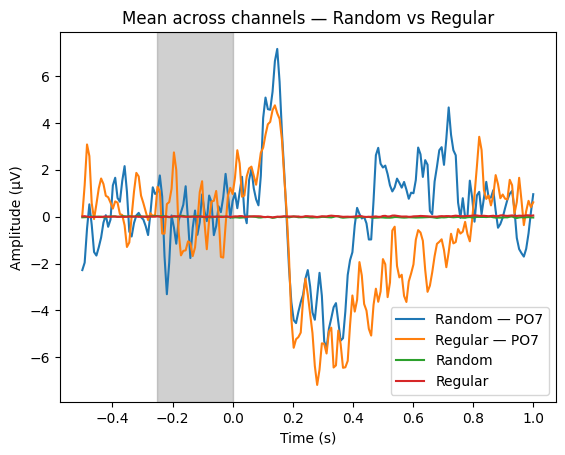
\includegraphics[width=1.1\linewidth]{assets/subject005/sub-005_all_channel_erp-2-noasr.png}
        \captionof{figure}{Subject 005 - Config 2 All Channels ERP (without ASR)}
        \label{fig:sub005-all-erp-2}
    \end{minipage}
\end{figure}


\subsubsection{ICA interaction with ASR}
The ICA topographies for subject 005 shows a significant difference between the two pipelines.

\begin{figure}[!h]
    \centering
    \hspace{-1.5cm}\begin{minipage}{.48\textwidth}
        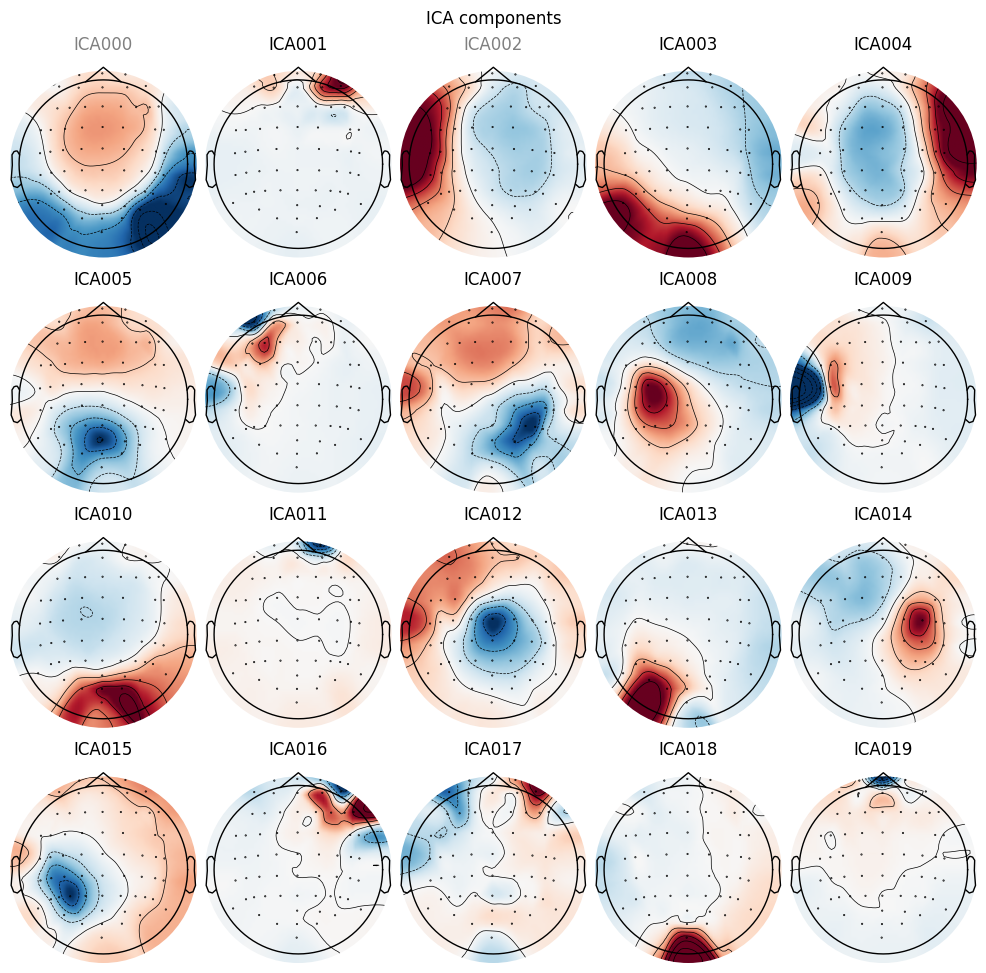
\includegraphics[width=1.2\linewidth]{assets/subject005/sub-005_ica-1-default.png}
        \captionof{figure}{Subject 005 - Config 1 ICA (with ASR)}
        \label{fig:sub005-ica-1}
    \end{minipage}\hspace{1.7cm}
    \begin{minipage}{.48\textwidth}
        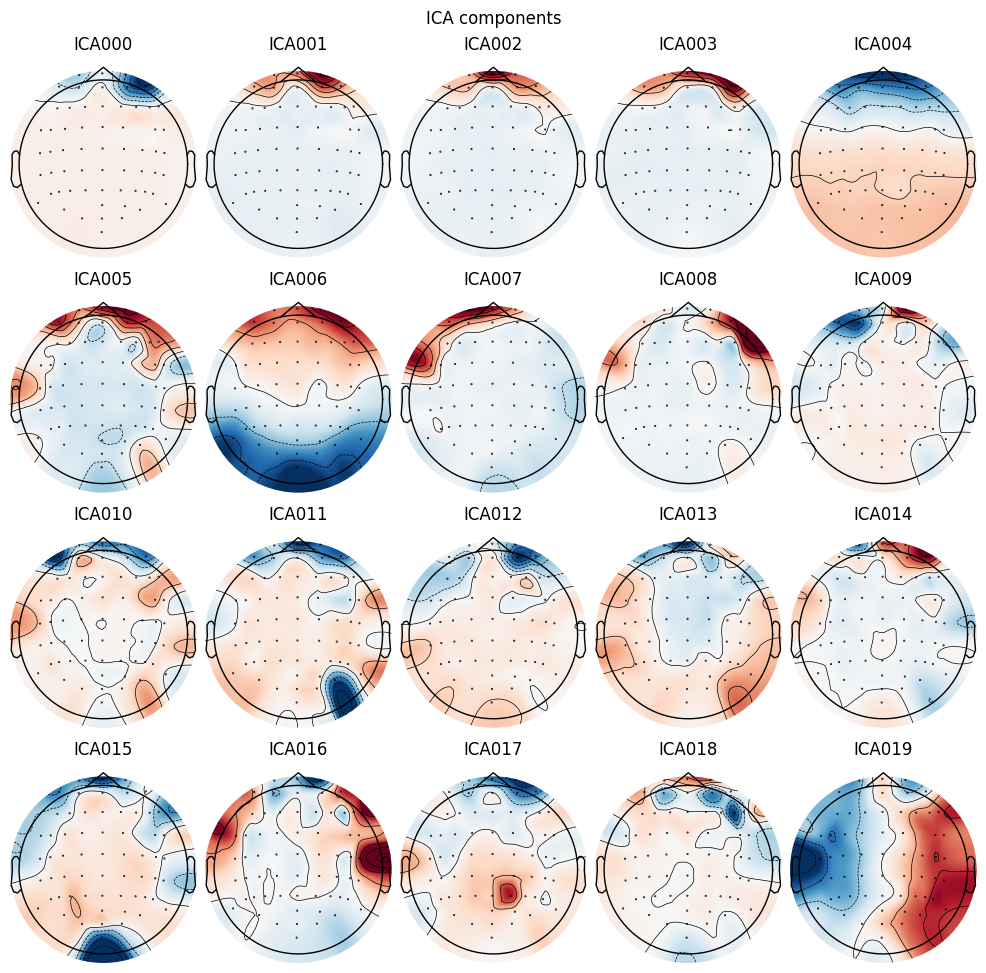
\includegraphics[width=1.2\linewidth]{assets/subject005/sub-005_ica-2-noasr.png}
        \captionof{figure}{Subject 005 - Config 2 ICA (without ASR)}
        \label{fig:sub005-ica-2}
    \end{minipage}
\end{figure}
 Without ASR (Figure \ref{fig:sub005-ica-2}), the first several components (ICA000–ICA004) show frontal-dominant patterns with strong activity concentrated at the frontal electrodes, which is the classic signature of eye blink and eye movement artifacts. These are clear, well-separated components that the automatic detection can identify and remove. With ASR enabled (Figure \ref{fig:sub005-ica-1}), the frontal blink patterns are largely absent from the leading components as ASR has already removed the blink-related signal before ICA sees it. Instead, the leading components show broader, more distributed topographies that are harder to classify as artifact or neural.


\subsubsection{Summary}
Ordering the steps by their impact on the final result for this subject gives us:
\begin{enumerate}
    \item filtering provides the largest improvement in raw signal quality by removing high-frequency noise and line interference
    \item re-referencing has the second-largest effect by removing shared noise and providing a physically meaningful reference
    \item ASR has the largest effect on ERP morphology, but in a detrimental direction for our specific analysis by attenuating the SPN
    \item bad channel detection has a minor but positive impact by removing outlier channels
    \item ICA's impact depends heavily on whether ASR was applied first, with more pronounced artifact removal when ASR is absent
\end{enumerate}



\section{Summary}
In this report, we developed a fully automated EEG preprocessing pipeline to replicate the ERP findings of Makin et al. \cite{paper} on visual symmetry perception. Our pipeline replaced all manual steps with automatic alternatives: variance and correlation-based bad channel detection, bandpass and notch filtering, downsampling, average re-referencing, ASR, ICA with automatic component identification, spherical spline interpolation, epoching with baseline correction, and amplitude-based trial rejection. Using TOML-based configuration files, we could flexibly enable, disable, and parameterize each step, allowing systematic comparison of different pipeline configurations across all 24 subjects.
Our pipeline successfully reproduced the general ERP morphology at PO7/PO8, including the P1 and N1 components. However, the sustained posterior negativity (SPN), the primary marker of symmetry perception, was substantially attenuated when ASR was enabled. Disabling ASR recovered the SPN, closely matching the authors' results. We investigated this discrepancy through automatic blink detection on the EOG channels and found that blink-contaminated epochs show a larger ASR-induced difference than blink-free epochs, suggesting that blink removal by ASR contributes to the SPN attenuation. However, differences persist even in blink-free epochs, indicating that ASR also removes other signal components that contribute to the SPN. Our step-by-step analysis further revealed that re-referencing and filtering have the largest positive impact on data quality, while bad channel detection and interpolation have comparatively minor effects on the grand average.

\section{Conclusion}
Our replication demonstrates that the key ERP findings of Makin et al. \cite{paper}, particularly the sustained posterior negativity for reflectional symmetry, are robust and reproducible with a fully automated pipeline, provided that ASR is not included. The addition of ASR, which we initially expected to improve data quality, instead attenuated the very effect we aimed to replicate.
This finding carries a practical lesson for ERP research: artifact correction methods designed for transient, high-amplitude artifacts can interfere with sustained, low-frequency ERP components when the two share temporal or spectral characteristics. The SPN is a slow, sustained negativity extending over hundreds of milliseconds. Precisely the kind of signal that ASR's subspace reconstruction may partially absorb, especially when blink artifacts in the same time window trigger correction. This aligns with the broader argument made by Delorme \cite{leftalone} that aggressive automated preprocessing does not always improve ERP outcomes and can sometimes degrade them.
For future work, several avenues could be explored. Running ASR only on EEG channels (excluding EOG) might reduce the interaction between blink correction and posterior ERP signals. Alternatively, applying ASR with a higher cutoff or restricting it to specific frequency bands could preserve more of the sustained neural activity. A more targeted approach would be to use ICA alone for blink removal — as the authors did — rather than relying on ASR's broader subspace correction. Finally, our blink analysis could be strengthened with formal statistical testing (e.g., permutation tests on the SPN amplitude difference between blink and non-blink epochs) rather than the visual comparison we performed here.
Overall, our work highlights the importance of systematically evaluating each preprocessing step's impact on the specific ERP components of interest, rather than assuming that more cleaning necessarily leads to better results.

\newpage
\printbibliography[
    heading=bibintoc,
    title={References}
]

\end{document}